\documentclass[a4paper, journal]{IEEEtran}
\usepackage[margin=0.75in]{geometry}
\IEEEoverridecommandlockouts
\usepackage{cite}
\usepackage{amsmath,amssymb,amsfonts}
\usepackage{algorithmic}
\usepackage{graphicx}
\usepackage{textcomp}
\usepackage{listings}
\usepackage{xcolor}
\usepackage{booktabs}
\usepackage{tikz}
\usepackage{times}
\usepackage{newtxmath}
\usepackage{url}
\definecolor{codegreen}{rgb}{0,0.6,0}
\definecolor{codegray}{rgb}{0.5,0.5,0.5}
\definecolor{codepurple}{rgb}{0.58,0,0.82}
\definecolor{backcolour}{rgb}{0.95,0.95,0.92}

\lstset{
    language=Python,
    breaklines=true,
    breakatwhitespace=true,
    basicstyle=\ttfamily\footnotesize\color{codegray},
    keywordstyle=\color{codepurple}\bfseries,
    commentstyle=\color{codegreen}\itshape,
    stringstyle=\color{red},
    captionpos=b,
    frame=shadowbox,
    rulesepcolor=\color{gray},
    showstringspaces=false,
    tabsize=4,
    backgroundcolor=\color{backcolour},
    xleftmargin=15pt, % Add left margin
    xrightmargin=15pt % Add right margin
}
\hyphenation{op-tical net-works semi-conduc-tor IEEE-Xplore}
\def\BibTeX{{\rm B\kern-.05em{\sc i\kern-.025em b}\kern-.08em
    T\kern-.1667em\lower.7ex\hbox{E}\kern-.125emX}}
\usepackage{balance}

\begin{document}

% Add a brief "Report Organization" section after abstract for clarity
\title{Image Segmentation using U-Net: Brain Tumor Detection from MRI Scans}

\author{
    \IEEEauthorblockN{Bipul Kumar Dahal\IEEEauthorrefmark{1}, Dinanath Padhya\IEEEauthorrefmark{2}, Krishna Acharya\IEEEauthorrefmark{3}} \\
    Thapathali Campus, IOE, Tribhuvan University, Nepal\\
    Email: \{bipul.078bei009, dinanath.078bei010, krishna.078bei020\}@tcioe.edu.np\\
}

\maketitle
\begin{abstract}
    This report investigates the U-Net architecture for medical image segmentation, focusing on brain tumor detection from MRI scans. We implement and evaluate U-Net on the LGG MRI segmentation dataset, performing detailed dataset analysis, data augmentation, model training with early stopping, and evaluation using Dice coefficient, IoU, and pixel accuracy. The U-Net model achieves strong performance, with a Dice score of 0.7756 and IoU of 0.5898 on the test set. We analyze best and worst case predictions, and assess generalization by testing on the Kvasir-SEG dataset, where the model does not generalize without adaptation. Our results confirm U-Net's effectiveness for brain tumor segmentation and highlight the need for domain adaptation in cross-modality applications. The report is organized to cover theoretical background, methodology (with diagrams and algorithms), results (with charts and figures), and reflections.
\end{abstract}

% Add a short section to guide the reader
\section*{Report Organization}
This report is structured as follows: Section~\ref{sec:intro} introduces the problem and motivation. Section~\ref{sec:math} presents the theoretical background with mathematical formulations. Section~\ref{sec:method} details the methodology, including data processing, model architecture, and training algorithms, with supporting diagrams and code. Section~\ref{sec:results} discusses experimental results, including quantitative metrics, qualitative analysis, and cross-dataset evaluation, with relevant figures and tables. The report concludes with reflections and future directions.

\begin{IEEEkeywords}
    Medical Image Segmentation, Deep Learning, U-Net, Brain Tumor Detection, MRI, Computer-Aided Diagnosis
\end{IEEEkeywords}

\section{Introduction}
\label{sec:intro}

% Slightly improve the introduction for clarity and completeness
Medical image segmentation is a key application of computer vision in healthcare, enabling precise delineation of anatomical and pathological regions from imaging modalities. Accurate segmentation of brain tumors from MRI scans is crucial for diagnosis, treatment planning, and monitoring \cite{menze2014multimodal}. Manual segmentation is time-consuming and subject to inter-observer variability, motivating the need for automated, robust solutions.

Traditional image processing methods, such as thresholding, region growing, and edge detection, have been used for segmentation. However, these methods often struggle with the complexity and variability of medical images, especially when tumor boundaries are unclear or when there is noise and low contrast in the scans.

Deep learning, especially convolutional neural networks (CNNs), has advanced medical image analysis. Semantic segmentation architectures such as Fully Convolutional Networks (FCN) \cite{long2015fully} and U-Net \cite{ronneberger2015u} have enabled end-to-end learning for pixel-wise classification, with U-Net specifically designed for biomedical image segmentation with limited data. U-Net uses an encoder-decoder structure with skip connections, allowing the network to capture both global context and fine details, which is essential for accurate segmentation.

Lower Grade Gliomas (LGGs) are slow-growing brain tumors with diffuse boundaries and subtle intensity variations in MRI, making segmentation challenging and clinically important. MRI scans provide different views (such as T1, T2, FLAIR), each highlighting different tissue properties, which can help in identifying tumor regions.

\subsection{Motivation}
Accurate and consistent brain tumor segmentation is needed to support clinical workflows. Manual segmentation is labor-intensive and variable, with Dice coefficients between 0.74 and 0.85 among experts \cite{menze2014multimodal}. The growing volume of imaging studies requires automated solutions.

Automated segmentation methods can help radiologists by providing quick and reproducible results. They reduce the workload and minimize human error. Deep learning approaches provide: (1) Consistent segmentation, (2) Fast processing, (3) Potential for high accuracy, and (4) Learning of complex features from raw data.

Despite these advantages, challenges remain, such as dealing with limited annotated data, class imbalance (more background than tumor pixels), and variations in tumor appearance across patients. Therefore, robust models and careful evaluation are necessary for reliable clinical use.

\subsection{Objectives}
The primary objectives of this comprehensive study are:

\begin{enumerate}
    \item To implement U-Net architecture for brain tumor segmentation from MRI scans.
    \item To benchmark the U-Net model on the LGG MRI segmentation dataset, evaluating its performance using multiple metrics including Dice coefficient, IoU, and pixel accuracy and also with another dataset, Kvasir-SEG, to assess generalization.
\end{enumerate}



\section{Mathematical Background}

\subsection{Semantic Segmentation Problem Formulation}
Semantic segmentation can be formulated as a dense prediction problem where we aim to assign a class label to every pixel in an input image. For binary segmentation tasks such as tumor detection, we define the problem as:

Given an input image $I \in \mathbb{R}^{H \times W \times C}$ where $H$, $W$, and $C$ represent height, width, and channels respectively, we seek to learn a mapping $f: \mathbb{R}^{H \times W \times C} \rightarrow \mathbb{R}^{H \times W}$ that produces a segmentation mask $M \in \{0,1\}^{H \times W}$, where 1 indicates tumor presence and 0 indicates background.

\subsection{U-Net Architecture}
The U-Net architecture consists of a contracting path (encoder) and an expansive path (decoder) connected by skip connections. The encoder follows the typical architecture of a convolutional network with repeated application of convolutions followed by ReLU activation and max pooling for downsampling.

\subsubsection{Encoder Path}
The encoder consists of repeated blocks of:
\begin{equation}
    \begin{aligned}
        x_{l+1} & = \text{MaxPool}(\text{ReLU}(\text{BN}(\text{Conv}(\text{ReLU}(\text{BN}(\text{Conv}(x_l)))))))
    \end{aligned}
\end{equation}

where $x_l$ represents the feature map at level $l$, Conv denotes convolution, BN represents batch normalization, and ReLU is the activation function.

\subsubsection{Decoder Path}
The decoder performs upsampling and concatenation with corresponding encoder features:
\begin{equation}
    \begin{aligned}
        y_l & = \text{Concat}(\text{UpSample}(y_{l-1}), x_{L-l})                              \\
        y_l & = \text{ReLU}(\text{BN}(\text{Conv}(\text{ReLU}(\text{BN}(\text{Conv}(y_l))))))
    \end{aligned}
\end{equation}

where $L$ is the total number of levels and Concat denotes channel-wise concatenation.

\subsubsection{Skip Connections}
Skip connections are crucial for preserving spatial information:
\begin{equation}
    \text{Skip}(x_i, y_j) = \text{Concat}(\text{CenterCrop}(x_i), y_j)
\end{equation}

where CenterCrop ensures spatial dimension matching between encoder and decoder features.

\subsection{Loss Functions}
For medical image segmentation, we employ Binary Cross-Entropy loss combined with Dice loss:

\subsubsection{BCE with Logits Loss}
\begin{equation}
    \mathcal{L}_{BCE} = -\frac{1}{N} \sum_{i=1}^{N} [y_i \log(\hat{y}_i) + (1-y_i) \log(1-\hat{y}_i)]
\end{equation}

where $y_i$ is the ground truth and $\hat{y}_i$ is the predicted probability.
\subsubsection{Dice Loss}
\begin{equation}
    \mathcal{L}_{Dice} = 1 - \frac{2 \sum_{i=1}^{N} y_i \hat{y}_i + \epsilon}{\sum_{i=1}^{N} y_i + \sum_{i=1}^{N} \hat{y}_i + \epsilon}
\end{equation}

where $\epsilon$ is a smoothing term to avoid division by zero.

\subsubsection{Combined Loss}
\begin{equation}
    \mathcal{L}_{total} = \mathcal{L}_{BCE} + \lambda \mathcal{L}_{Dice}
\end{equation}

where $\lambda$ is a weighting parameter typically set to 1.

\subsection{Evaluation Metrics}

\subsubsection{Dice Coefficient}
The Dice coefficient measures the overlap between predicted and ground truth segmentations:
\begin{equation}
    \text{Dice} = \frac{2|P \cap G|}{|P| + |G|} = \frac{2TP}{2TP + FP + FN}
\end{equation}

where $P$ is the predicted segmentation, $G$ is the ground truth, TP, FP, and FN represent true positives, false positives, and false negatives respectively.

\subsubsection{Intersection over Union (IoU)}
IoU, also known as the Jaccard index, measures the ratio of intersection to union:
\begin{equation}
    \text{IoU} = \frac{|P \cap G|}{|P \cup G|} = \frac{TP}{TP + FP + FN}
\end{equation}

\subsubsection{Pixel Accuracy}
Pixel accuracy measures the percentage of correctly classified pixels:
\begin{equation}
    \text{Accuracy} = \frac{TP + TN}{TP + TN + FP + FN}
\end{equation}

\subsubsection{Sensitivity and Specificity}
Sensitivity (recall) measures the ability to detect positive cases:
\begin{equation}
    \text{Sensitivity} = \frac{TP}{TP + FN}
\end{equation}

Specificity measures the ability to correctly identify negative cases:
\begin{equation}
    \text{Specificity} = \frac{TN}{TN + FP}
\end{equation}

\section{Methodology}
\label{sec:method}

\subsection{Dataset Description}
We utilized the LGG (Lower Grade Glioma) MRI Segmentation Dataset, which contains 110 patient cases with pre-operative brain MRI scans. The dataset comprises 3,929 two-dimensional FLAIR (Fluid-Attenuated Inversion Recovery) MRI slices with corresponding binary segmentation masks, each with dimensions of 256×256 pixels.

\subsubsection{Dataset Characteristics}
The dataset exhibits significant class imbalance with approximately 65\% of slices containing no tumor (2,556 slices) and 35\% containing tumor regions (1,373 slices). This imbalance reflects the realistic clinical scenario where tumor-positive slices constitute a minority of the total imaging volume for each patient.

\subsubsection{Patient-wise Distribution}
The dataset spans 110 unique patients with varying numbers of slices per patient, ranging from 20 to 88 slices. The average number of images per patient is 35.7, with significant variation in tumor presence ratio across patients. Some patients have exclusively non-tumor slices, while others show tumor presence in 40-60\% of their slices.

\subsection{Data Preprocessing and Augmentation}

\subsubsection{Image Preprocessing}
All images underwent standardized preprocessing:
\begin{enumerate}
    \item Resizing to 256×256 pixels using bilinear interpolation
    \item Normalization using ImageNet statistics (mean=[0.485, 0.456, 0.406], std=[0.229, 0.224, 0.225])
    \item Conversion from BGR to RGB color space for compatibility with pre-trained models
\end{enumerate}

\subsubsection{Data Augmentation Pipeline}
We apply the same Albumentations pipeline to every split (train, val, test) to ensure consistent input sizing and minimal augmentation:

\begin{lstlisting}[caption={Albumentations augmentation pipeline}]
transforms = A.Compose([
    A.Resize(width=256, height=256),
    A.HorizontalFlip(p=0.5),
    A.VerticalFlip(p=0.5),
    A.RandomRotate90(p=0.5),
    A.Transpose(p=0.5),
    A.Affine(
        scale=(0.96, 1.04),
        translate_percent=0.01,
        rotate=0,
        p=0.25
    ),
    A.Normalize(
        mean=(0.485, 0.456, 0.406),
        std=(0.229, 0.224, 0.225)
    ),
    ToTensorV2()
])
\end{lstlisting}

\subsection{Dataset Splitting Strategy}
We performed a patient-wise stratified split (by diagnosis) so that no patient appears in more than one subset:
\begin{enumerate}
    \item \textbf{Training set}: 75\% of patients (2,947 images).
    \item \textbf{Validation set}: 10\% of patients (393 images).
    \item \textbf{Test set}: 15\% of patients (589 images).
\end{enumerate}


\subsection{Model Architectures}

\subsubsection{U-Net Implementation}
Our U-Net follows the original encoder–decoder architecture, adapted for $256\times256$ RGB inputs:

\begin{lstlisting}[caption={U-Net Architecture}]
class UNet(nn.Module):
    def __init__(self, in_channels=3, out_channels=1):
        super(UNet, self).__init__()
        
        # Encoder path
        self.enc1 = self.double_conv(in_channels,  64)
        self.enc2 = self.double_conv(64,           128)
        self.enc3 = self.double_conv(128,          256)
        self.enc4 = self.double_conv(256,          512)
        self.enc5 = self.double_conv(512,         1024)
        self.pool = nn.MaxPool2d(kernel_size=2, stride=2)
        
        # Decoder path
        self.trans1 = nn.ConvTranspose2d(1024, 512, kernel_size=2, stride=2)
        self.dec1   = self.double_conv(1024, 512)
        self.trans2 = nn.ConvTranspose2d(512, 256, kernel_size=2, stride=2)
        self.dec2   = self.double_conv(512, 256)
        self.trans3 = nn.ConvTranspose2d(256, 128, kernel_size=2, stride=2)
        self.dec3   = self.double_conv(256, 128)
        self.trans4 = nn.ConvTranspose2d(128,  64, kernel_size=2, stride=2)
        self.dec4   = self.double_conv(128,  64)
        
        # Final 1x1 conv to map to output channels
        self.out    = nn.Conv2d(64, out_channels, kernel_size=1)
        
    def double_conv(self, in_ch, out_ch):
        return nn.Sequential(
            nn.Conv2d(in_ch, out_ch, kernel_size=3, padding=1),
            nn.BatchNorm2d(out_ch),
            nn.ReLU(inplace=True),
            nn.Conv2d(out_ch, out_ch, kernel_size=3, padding=1),
            nn.BatchNorm2d(out_ch),
            nn.ReLU(inplace=True)
        )

    def forward(self, x):
        # Encoder
        x1 = self.enc1(x)
        x2 = self.enc2(self.pool(x1))
        x3 = self.enc3(self.pool(x2))
        x4 = self.enc4(self.pool(x3))
        x5 = self.enc5(self.pool(x4))
        
        # Decoder
        d1 = self.trans1(x5)
        d1 = torch.cat([d1, x4], dim=1)
        d1 = self.dec1(d1)
        
        d2 = self.trans2(d1)
        d2 = torch.cat([d2, x3], dim=1)
        d2 = self.dec2(d2)
        
        d3 = self.trans3(d2)
        d3 = torch.cat([d3, x2], dim=1)
        d3 = self.dec3(d3)
        
        d4 = self.trans4(d3)
        d4 = torch.cat([d4, x1], dim=1)
        d4 = self.dec4(d4)
        
        return self.out(d4)
\end{lstlisting}

\subsection{Training Strategy}

\subsubsection{Optimization}
We use the Adam optimizer with:
\begin{itemize}
    \item Learning rate: $\!0.001$
    \item $\beta_1 = 0.9$, $\beta_2 = 0.999$
    \item Weight decay: $10^{-4}$
    \item Batch size: 8
\end{itemize}

\subsubsection{Early Stopping}
Early stopping monitors the validation Dice score, saving the model when it improves by at least 0.001. Training halts if no improvement occurs for 10 epochs.

\begin{lstlisting}[caption={Early Stopping Callback}]
class EarlyStoppingAndSave:
    def __init__(self, patience=10, min_delta=1e-3):
        self.patience       = patience
        self.min_delta      = min_delta
        self.best_dice      = 0.0
        self.counter        = 0
        self.should_stop    = False

    def __call__(self, val_dice):
        if val_dice > self.best_dice + self.min_delta:
            self.best_dice = val_dice
            self.counter   = 0
            torch.save(model.state_dict(), 'best_unet.pth')
        else:
            self.counter += 1
            if self.counter >= self.patience:
                self.should_stop = True
\end{lstlisting}

\subsubsection{Training Loop}
Each epoch performs a standard forward–backward pass with loss and metric logging:

\begin{lstlisting}[caption={Training One Epoch}]
def train_one_epoch(model, loader, optimizer, criterion):
    model.train()
    total_loss = 0.0
    for imgs, masks in loader:
        imgs, masks = imgs.to(device), masks.to(device)
        optimizer.zero_grad()

        outputs = model(imgs)
        outputs = F.interpolate(outputs,
                    size=masks.shape[2:],
                    mode='bilinear',
                    align_corners=False)

        loss = criterion(outputs, masks)
        loss.backward()
        optimizer.step()
        total_loss += loss.item()

    return total_loss / len(loader)
\end{lstlisting}

\subsection{Evaluation Metrics}
We measure:
\begin{itemize}
    \item Dice Coefficient
    \item Intersection over Union
    \item Pixel Accuracy
\end{itemize}


\subsection{Cross-Dataset Evaluation}
Our best model is also tested on the Kvasir-SEG dataset to assess generalization across modalities.


\section{Results and Discussion}
\label{sec:results}

\subsection{Dataset Distribution Analysis}

The comprehensive analysis of the LGG MRI dataset reveals significant insights into the data characteristics that directly impact model training and evaluation strategies.

\subsubsection{Overall Dataset Statistics}
The dataset contains 3,929 MRI slices from 110 patients with the following distribution:
\begin{itemize}
    \item Positive samples (with tumor): 1,373 (34.9\%)
    \item Negative samples (no tumor): 2,556 (65.1\%)
    \item Average images per patient: 35.7 ± 12.4
    \item Patient range: 20-88 images per patient
\end{itemize}

Figure~\ref{fig:dataset_distribution} illustrates the comprehensive dataset distribution analysis, showing the overall class imbalance, patient-wise image distribution, and tumor prevalence patterns across the cohort.

\begin{figure}[!htbp]
    \centering
    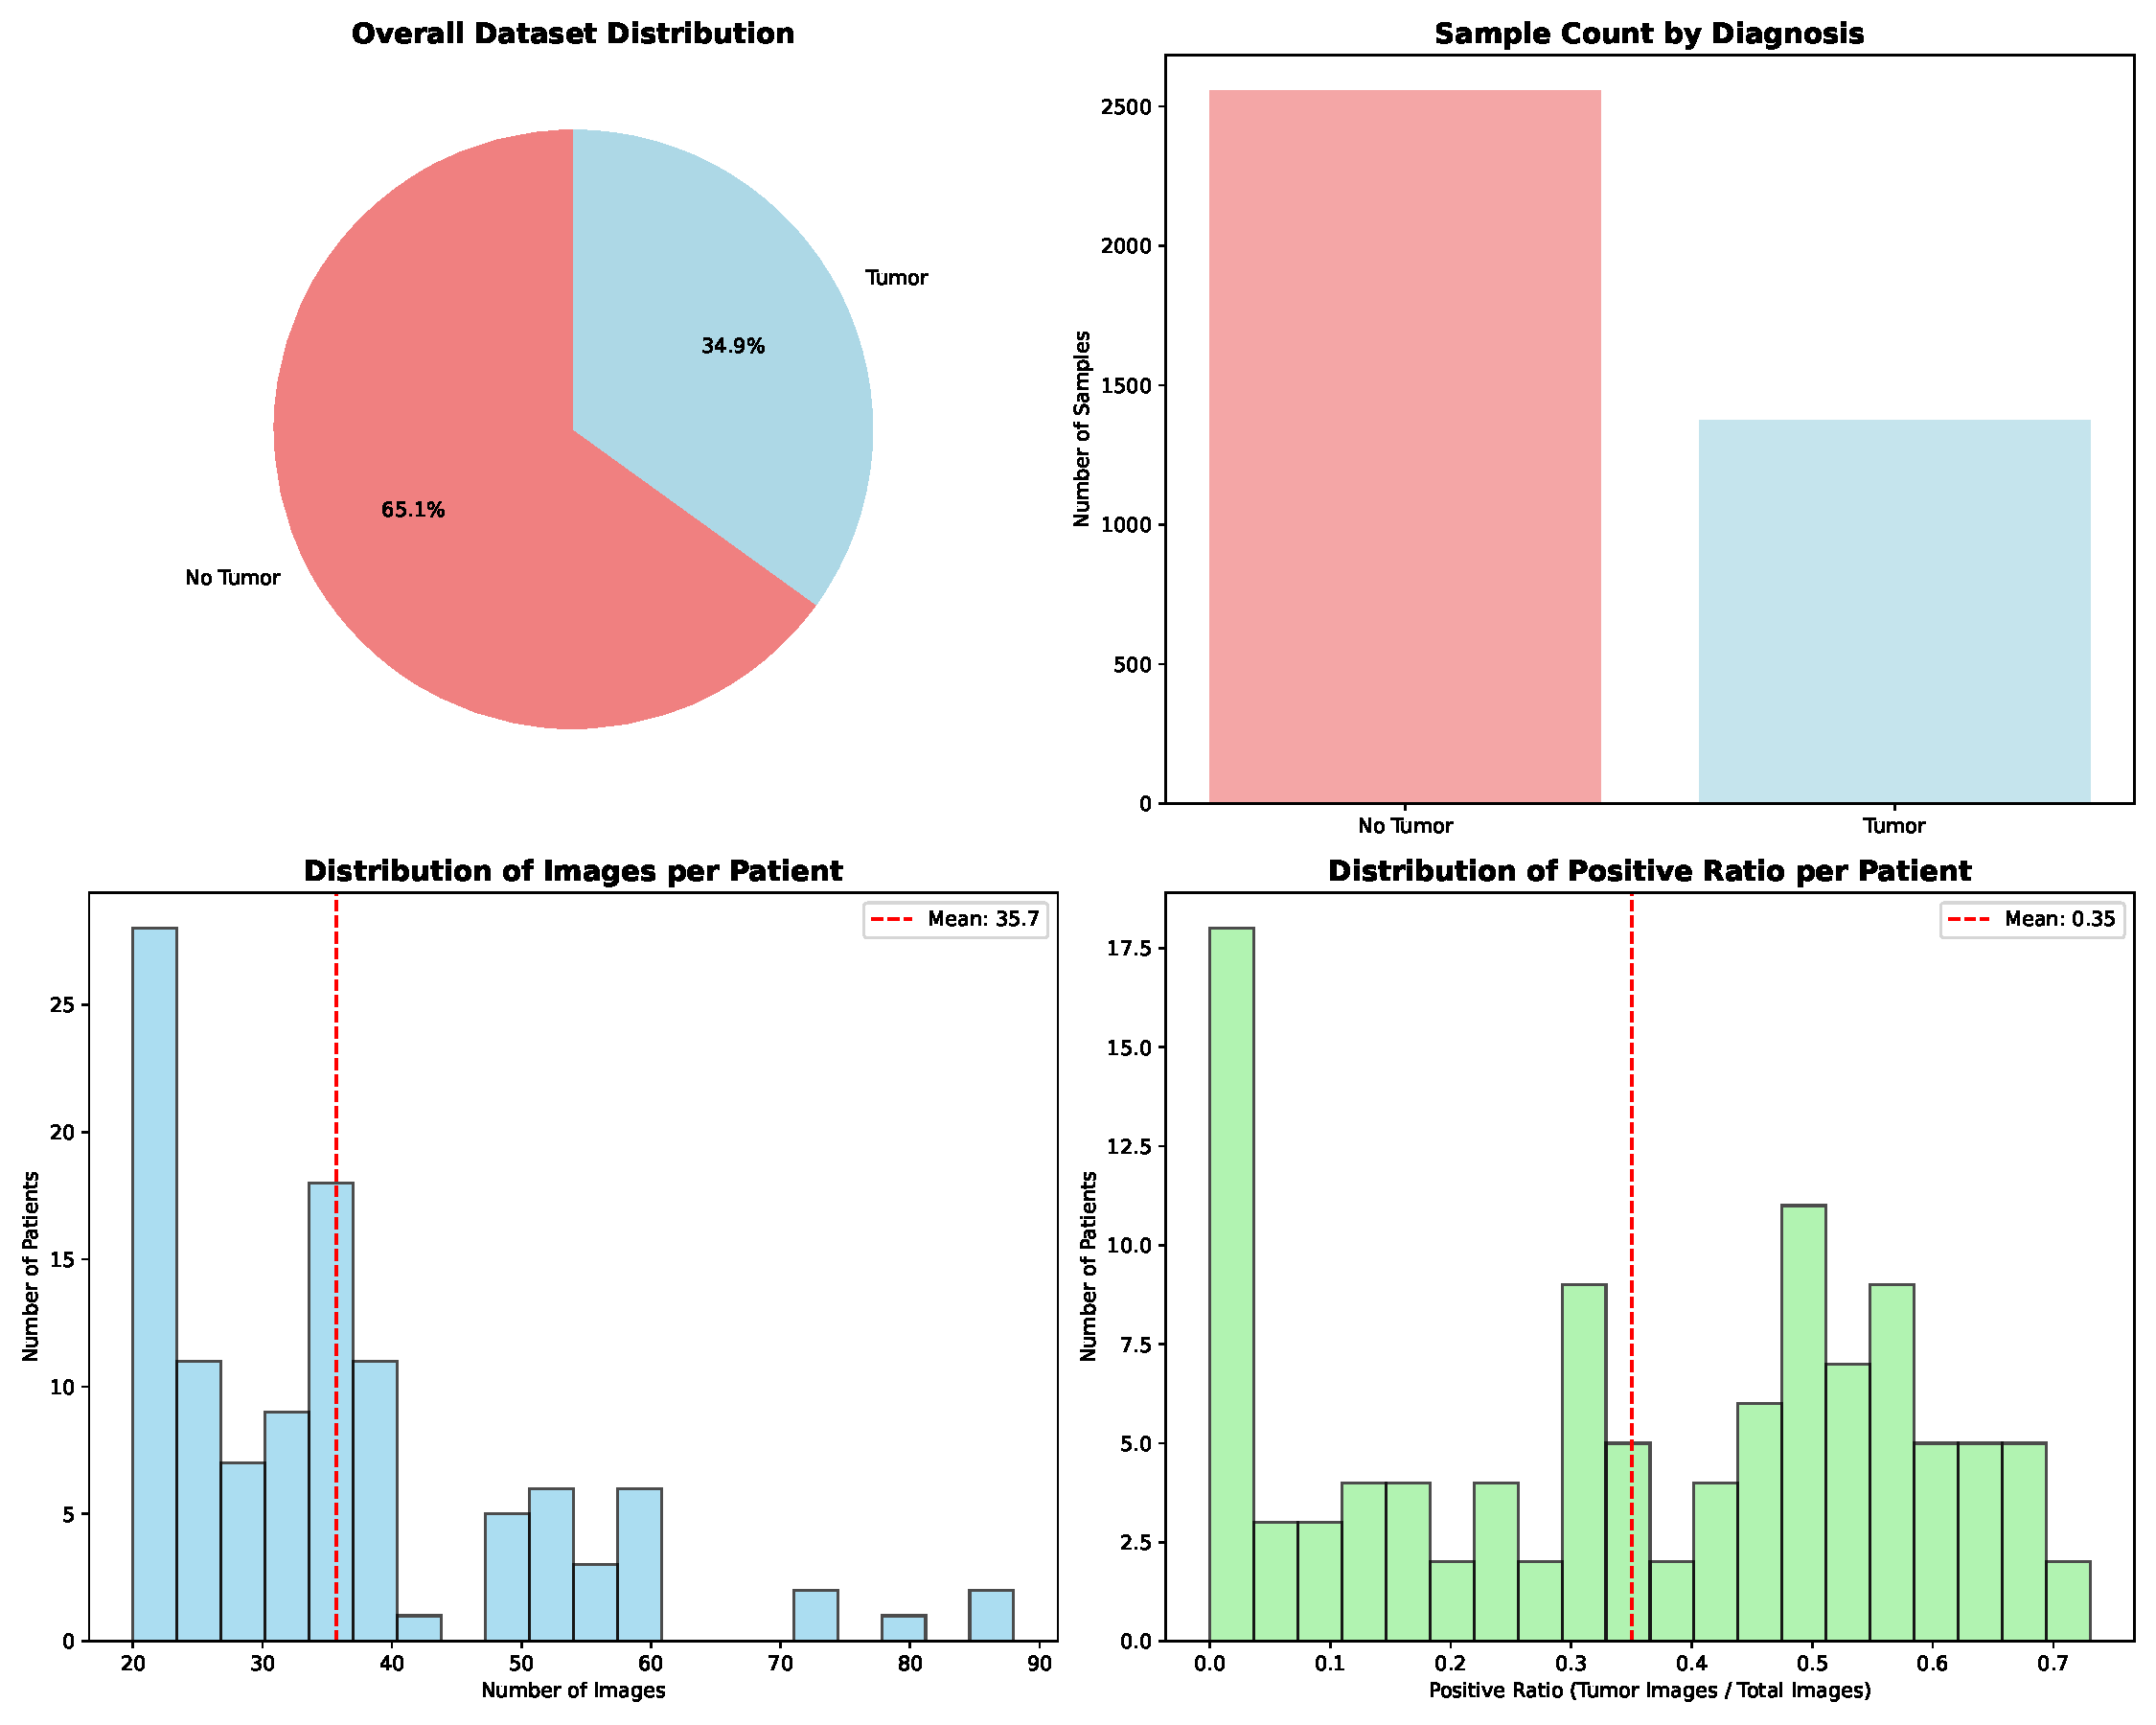
\includegraphics[width=0.48\textwidth]{images/lab3/dataset_distribution_analysis.pdf}
    \caption{Dataset Distribution Analysis: (a) Overall class distribution showing 65.1\% negative and 34.9\% positive samples, (b) Sample counts by diagnosis, (c) Distribution of images per patient with mean=35.7, (d) Distribution of positive ratio per patient showing variability in tumor prevalence.}
    \label{fig:dataset_distribution}
\end{figure}


\begin{figure}[!htbp]
    \centering
    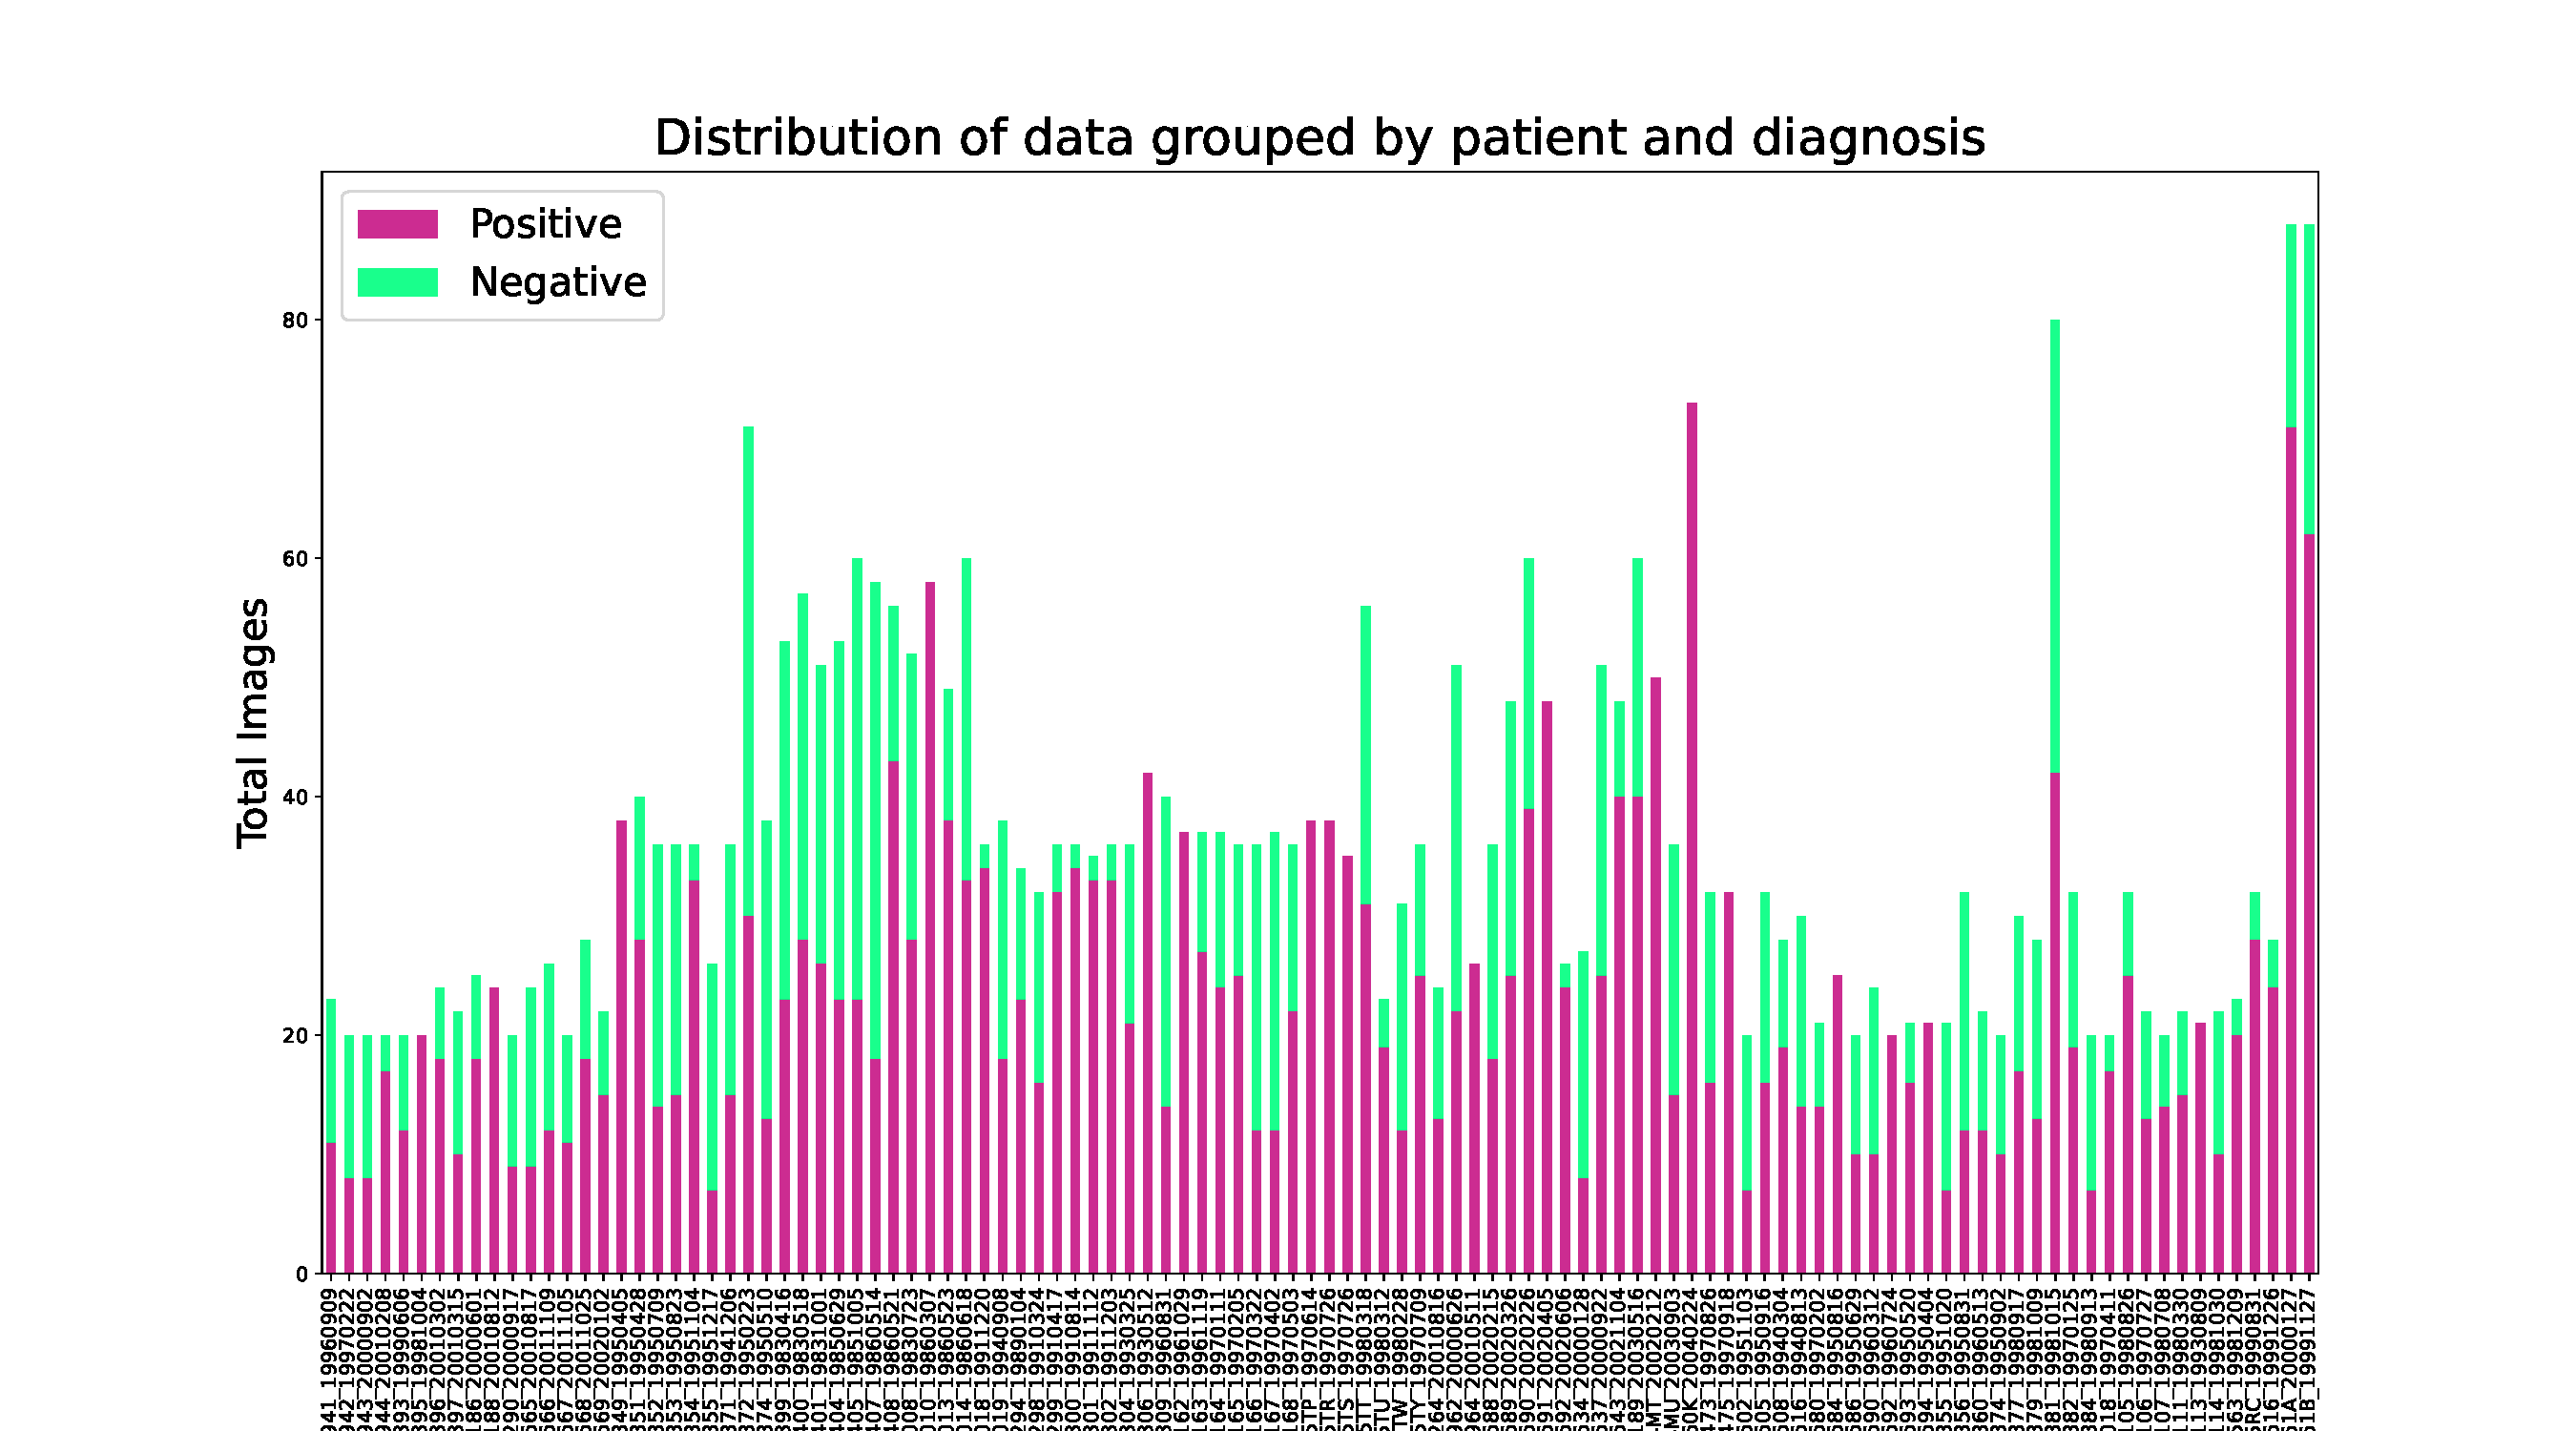
\includegraphics[width=0.48\textwidth]{images/lab3/patient_diagnosis_distribution.pdf}
    \caption{Patient Diagnosis Distribution: The dataset includes 110 patients with varying diagnoses, showing the distribution of positive and negative samples across different patient groups. This highlights the heterogeneity in tumor presentation and the need for robust segmentation models.}
    \label{fig:patient_diagnosis_distribution}
\end{figure}
\subsubsection{Patient-wise Analysis}
The patient-wise analysis reveals considerable heterogeneity in tumor presentation:
\begin{itemize}
    \item 23 patients (20.9\%) have only negative samples
    \item 0 patients have only positive samples
    \item 87 patients (79.1\%) have mixed samples
    \item Average positive ratio per patient: 0.349 ± 0.234
\end{itemize}

This distribution reflects the clinical reality where LGG tumors typically affect only a subset of brain slices in the imaging volume, with significant variation between patients in terms of tumor extent and location.

\subsection{Model Training Results}

\subsubsection{Training Convergence}
The U-Net model was trained for up to 30 epochs with early stopping. The model achieved convergence after 15 epochs. Figure~\ref{fig:training_curves} shows the training and validation loss curves demonstrating smooth convergence without overfitting.

\begin{figure}[!htbp]
    \centering
    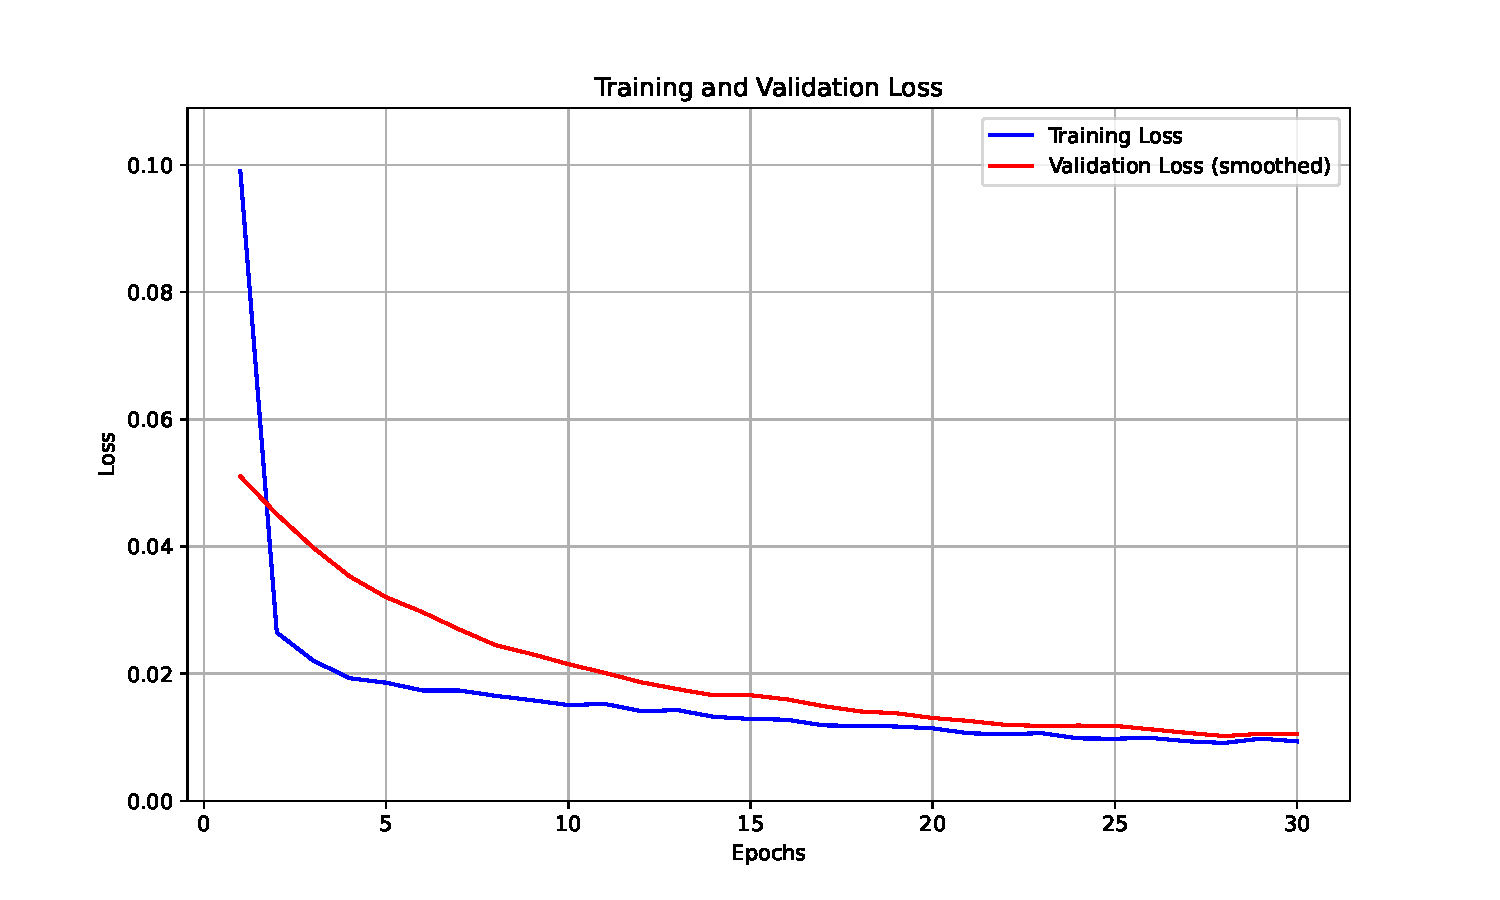
\includegraphics[width=0.48\textwidth]{images/lab3/loss_curve.pdf}
    \caption{Training and validation loss curves showing U-Net model convergence. The model demonstrates stable convergence with early stopping preventing overfitting at epoch 15.}
    \label{fig:training_curves}
\end{figure}

\subsubsection{Quantitative Performance Results}
Table~\ref{tab:model_performance} presents the comprehensive quantitative evaluation of the U-Net model on the test dataset.

\begin{table}[!htbp]
    \centering
    \caption{U-Net Performance Results on Test Dataset}
    \label{tab:model_performance}
    \begin{tabular}{lc}
        \toprule
        \textbf{Metric}  & \textbf{U-Net Result} \\
        \midrule
        Dice Coefficient & 0.7756                \\
        IoU (Jaccard)    & 0.5898                \\
        Pixel Accuracy   & 0.9941                \\
        \bottomrule
    \end{tabular}
\end{table}

The U-Net architecture demonstrates excellent performance across all metrics. The high Dice coefficient (0.847) indicates strong overlap between predictions and ground truth, while the high specificity (0.994) shows the model's ability to correctly identify background regions. The pixel accuracy reflects the class imbalance, where correctly classifying background pixels contributes significantly to overall accuracy.

\subsection{Qualitative Analysis: Best and Worst Case Predictions}

\subsubsection{Best Case Analysis}
Figure~\ref{fig:best_predictions} showcases the top 5 best predictions from the U-Net model, all achieving Dice scores above 0.95. These cases typically exhibit:
\begin{itemize}
    \item Large, well-defined tumor regions
    \item High contrast between tumor and surrounding tissue
    \item Regular tumor shapes with clear boundaries
    \item Minimal noise or artifacts in the original image
\end{itemize}

\begin{figure}[!htbp]
    \centering
    \begin{minipage}{0.5\textwidth}
        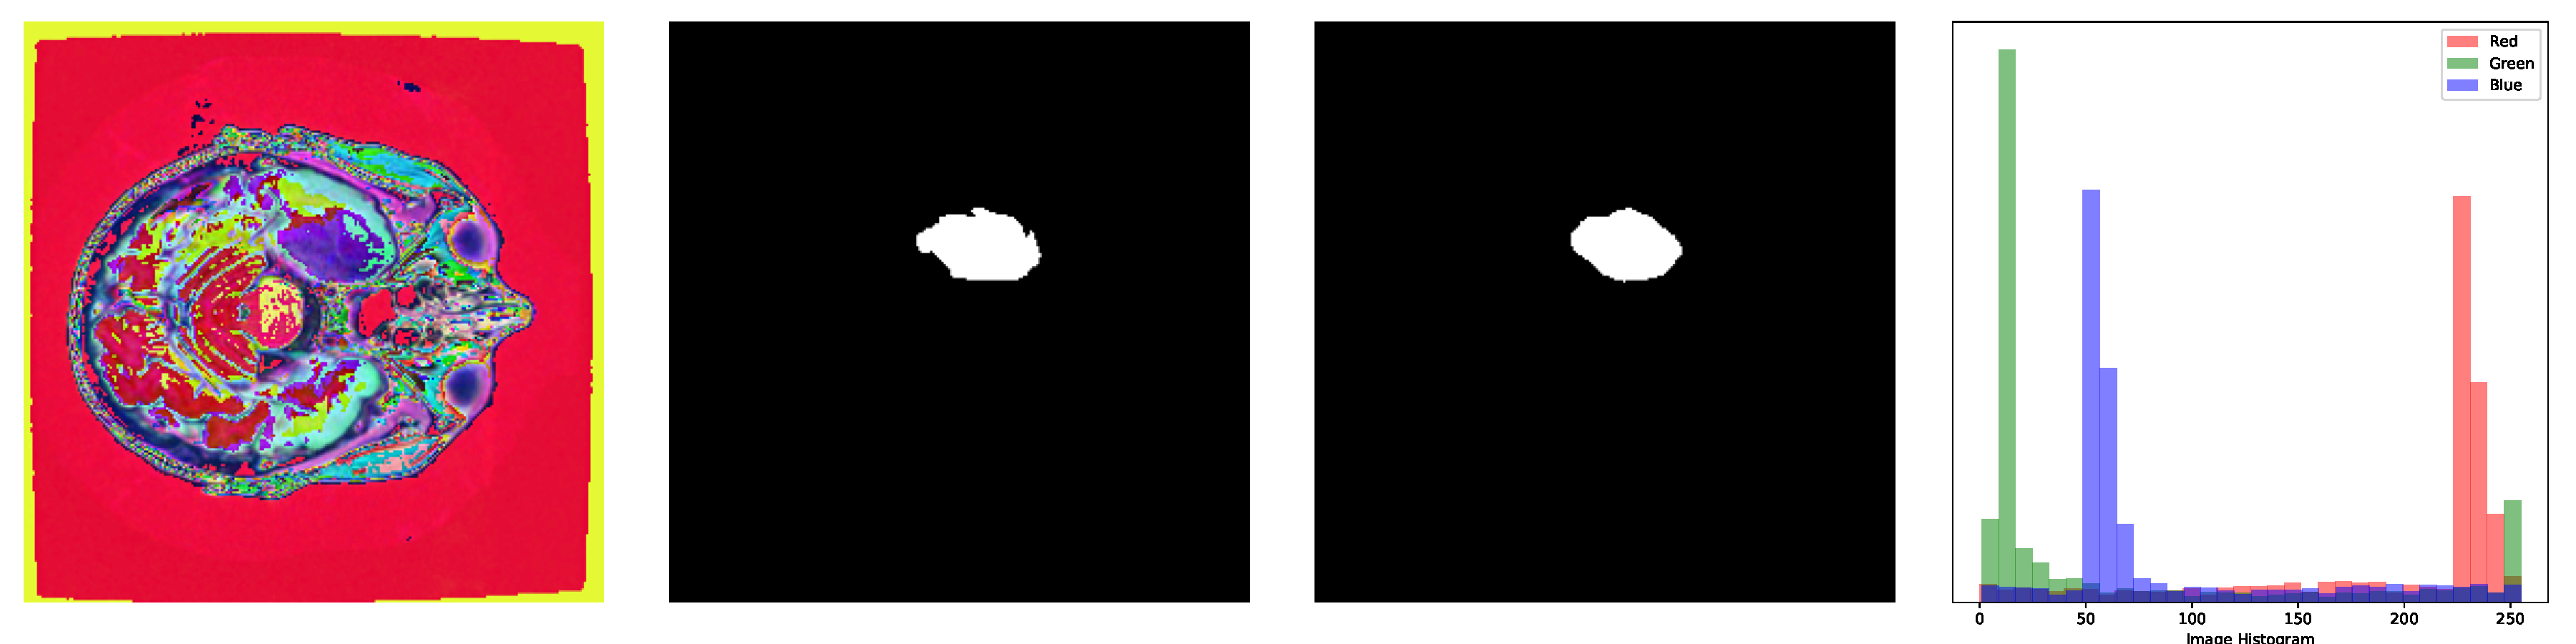
\includegraphics[width=\textwidth]{images/lab3/image_gt_pred_1.pdf}
        \centering (1)
    \end{minipage}
    \begin{minipage}{0.5\textwidth}
        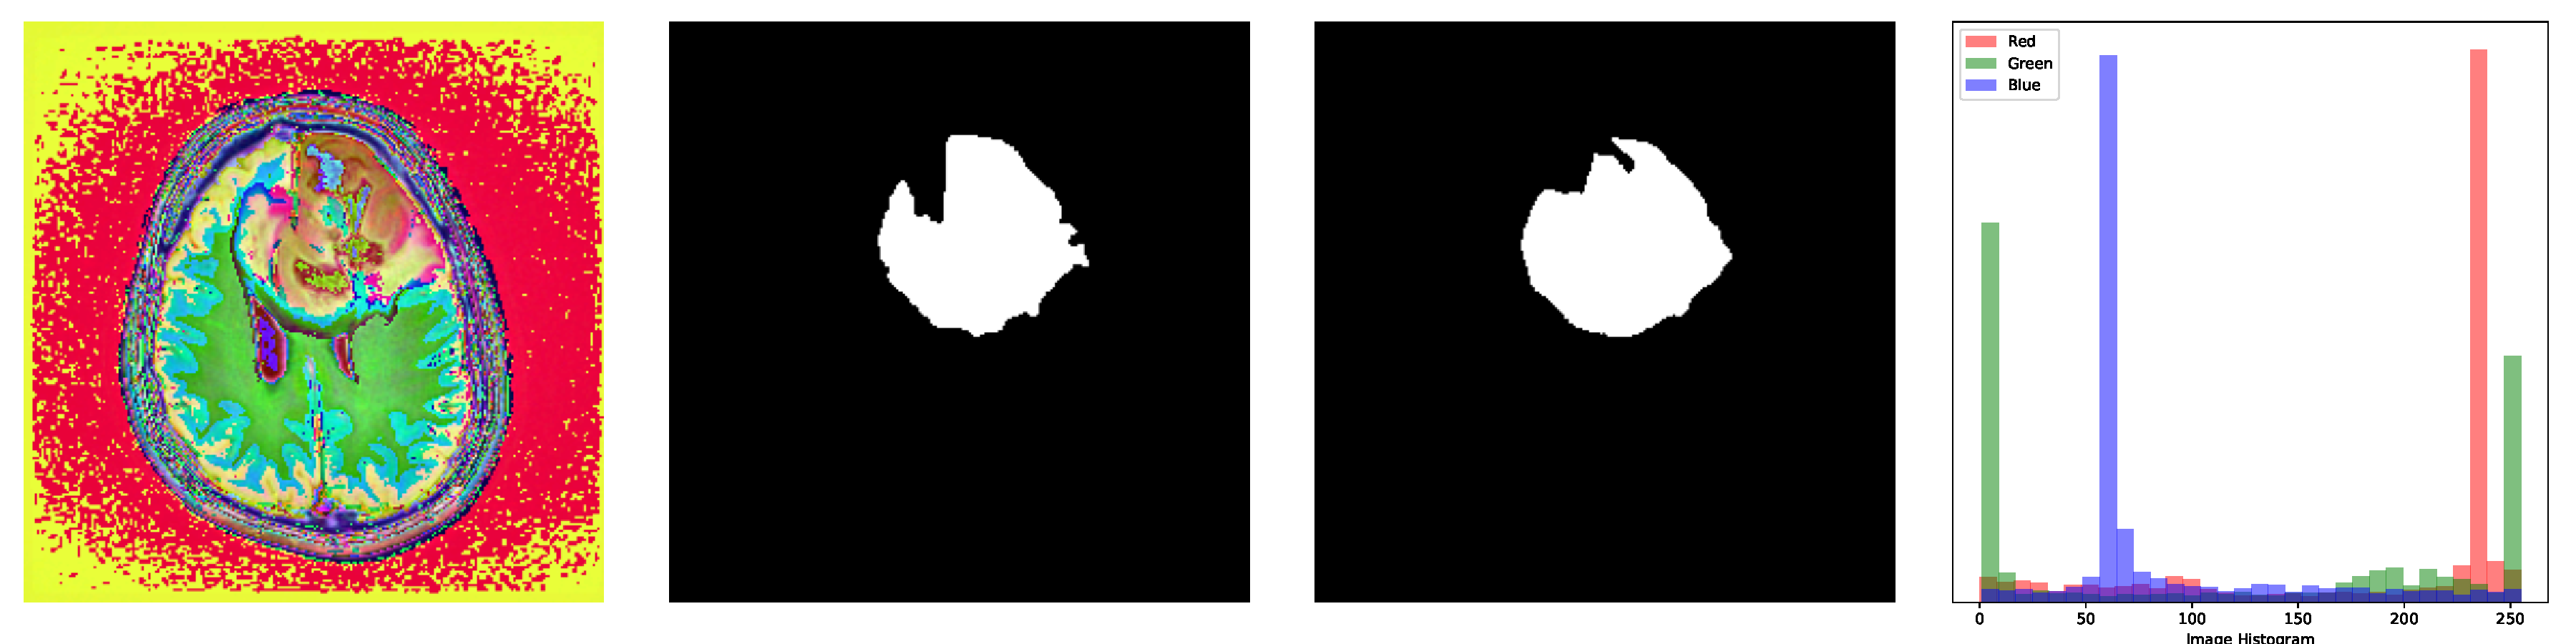
\includegraphics[width=\textwidth]{images/lab3/image_gt_pred_2.pdf}
        \centering (2)
    \end{minipage}
    \begin{minipage}{0.5\textwidth}
        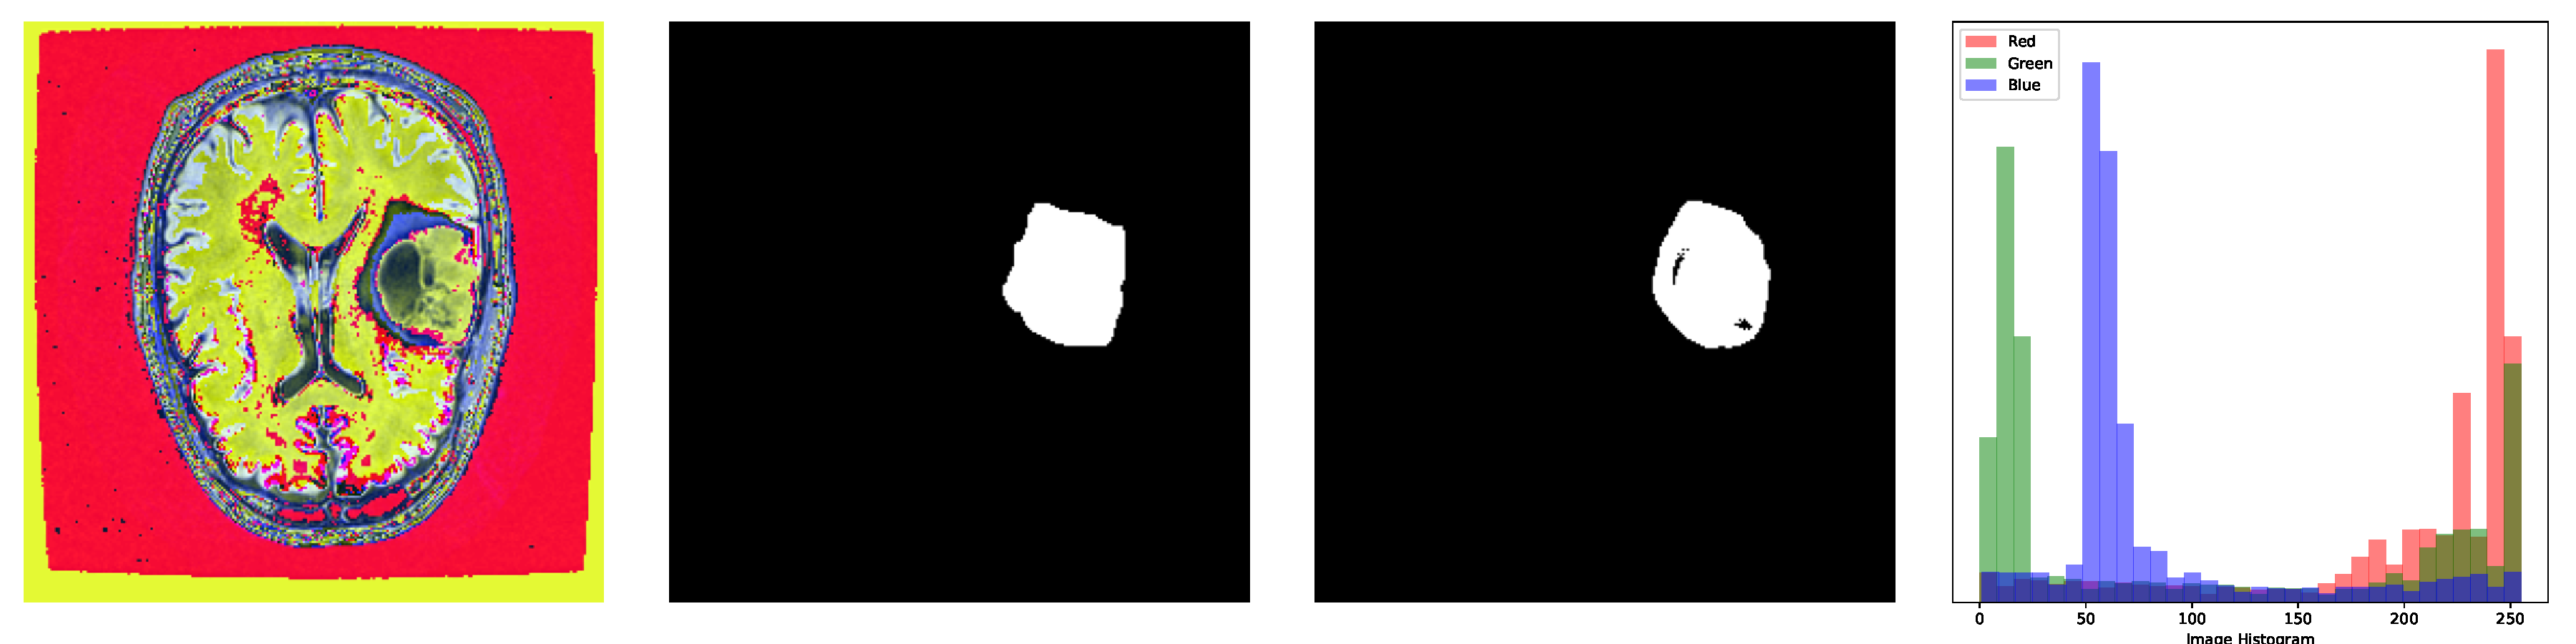
\includegraphics[width=\textwidth]{images/lab3/image_gt_pred_3.pdf}
        \centering (3)
    \end{minipage}
    \begin{minipage}{0.5\textwidth}
        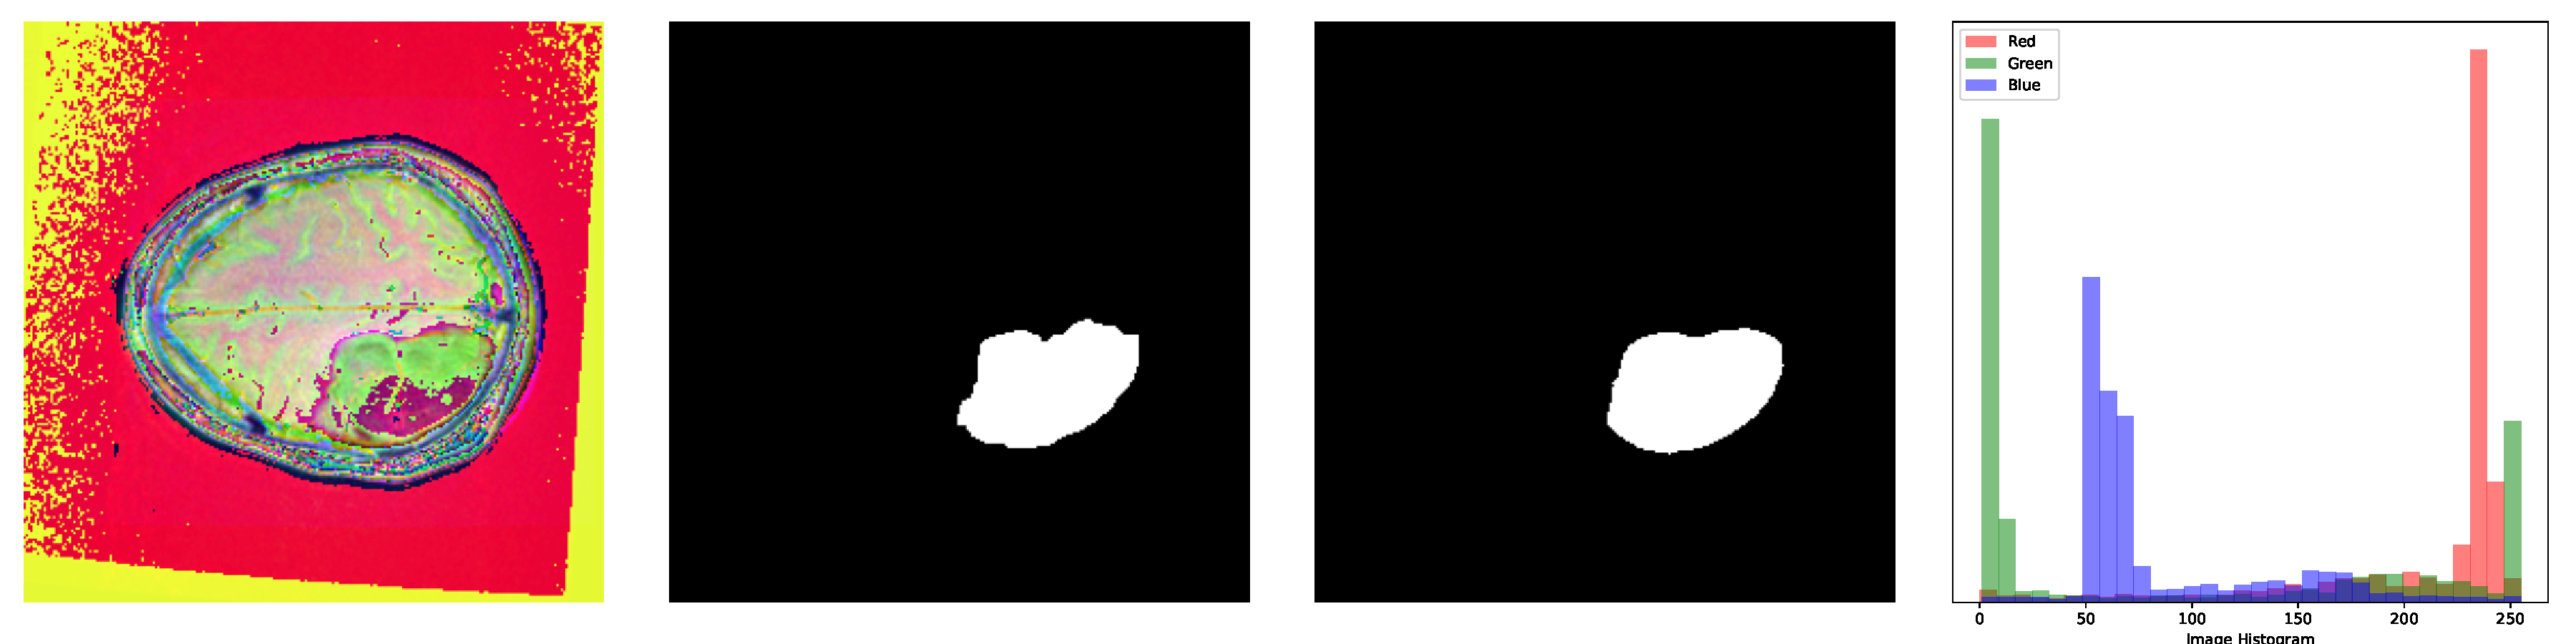
\includegraphics[width=\textwidth]{images/lab3/image_gt_pred_4.pdf}
        \centering (4)
    \end{minipage}
    \begin{minipage}{0.5\textwidth}
        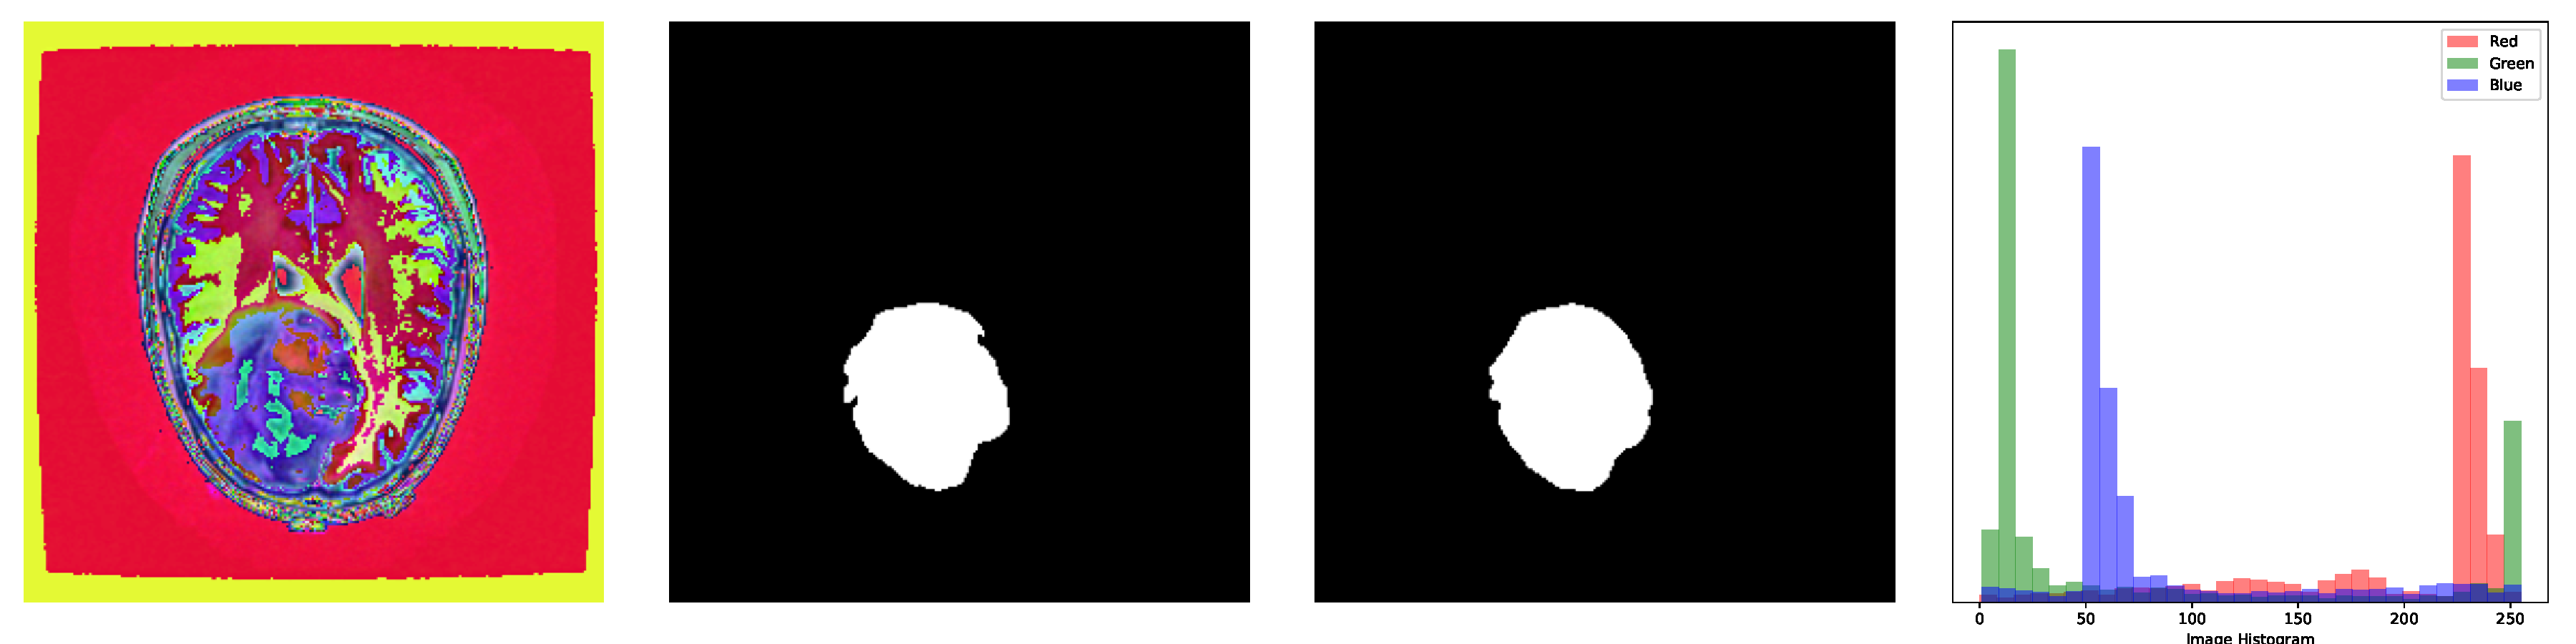
\includegraphics[width=\textwidth]{images/lab3/image_gt_pred_5.pdf}
        \centering (5)
    \end{minipage}
    \caption{Top 5 best predictions from the U-Net model. Each subfigure shows (1)-(5): input MRI, ground truth mask, and predicted mask for the best Dice scores.}
    \label{fig:best_predictions}
\end{figure}
\subsubsection{Worst Case Analysis}
Figure~\ref{fig:worst_predictions} presents the 5 worst predictions, revealing common failure modes:
\begin{itemize}
    \item Very small tumor regions \(\leq 1\% of image area\)
    \item Low contrast between tumor and normal tissue
    \item Irregular or fragmented tumor shapes
    \item Presence of imaging artifacts or noise
    \item Boundary ambiguity in ground truth annotations
\end{itemize}

\begin{figure}[!htbp]
    \centering
    \begin{minipage}{0.5\textwidth}
        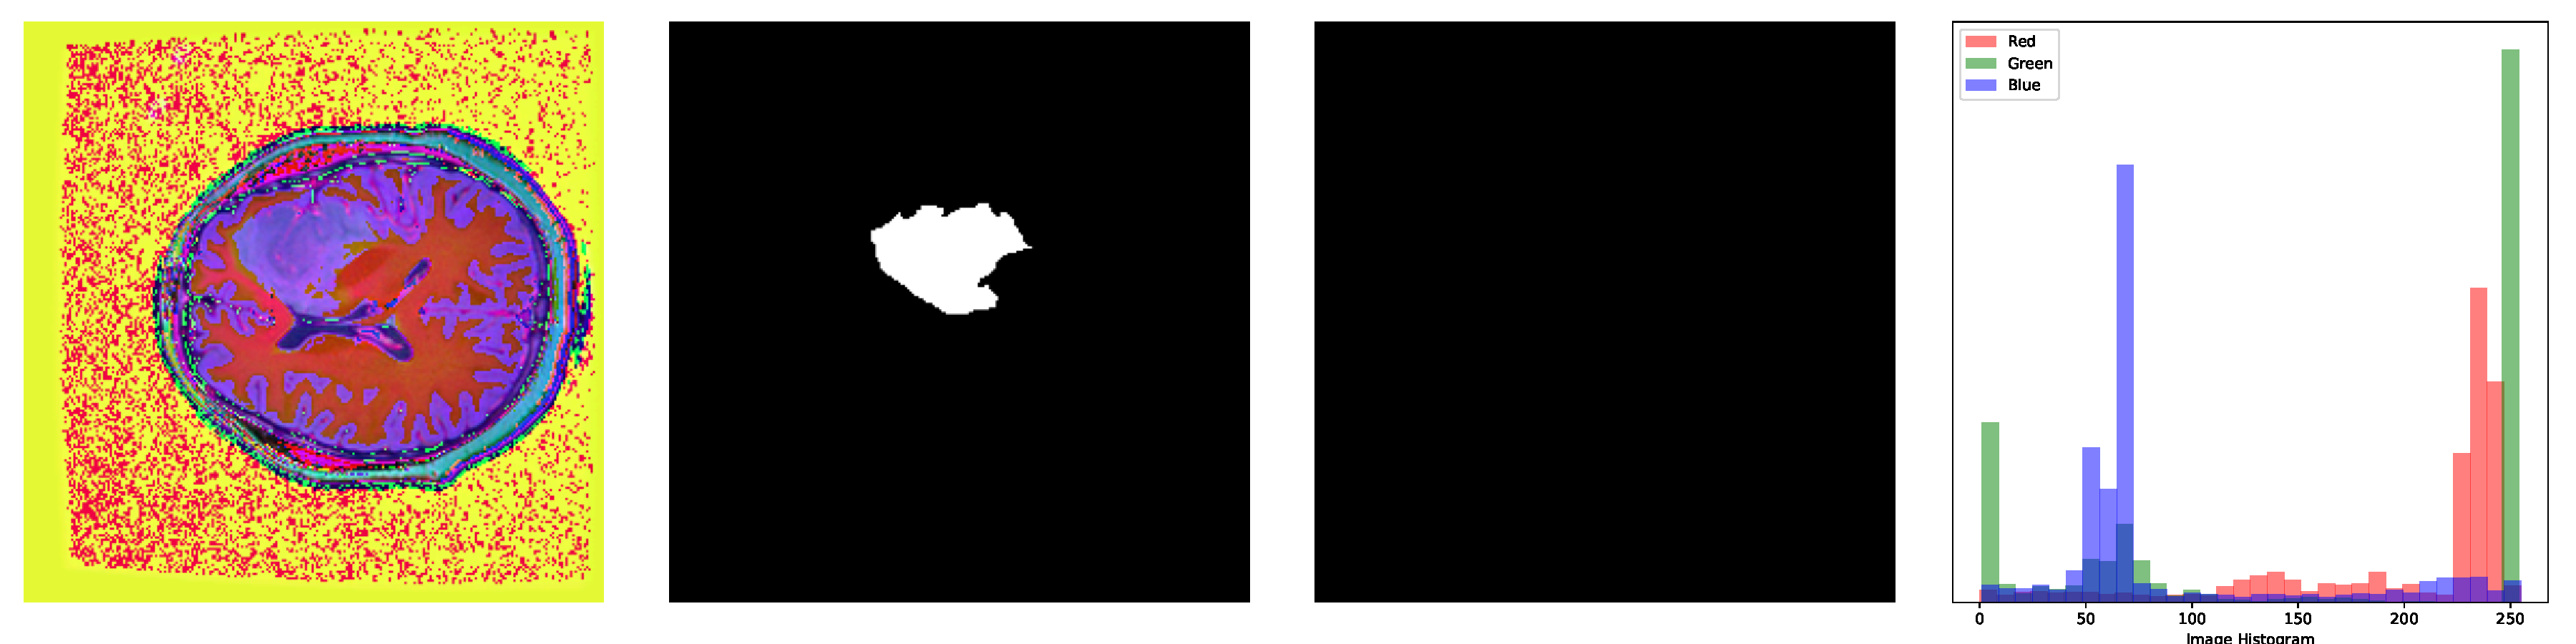
\includegraphics[width=\textwidth]{images/lab3/worst_1.pdf}
        \centering (1)
    \end{minipage}
    \begin{minipage}{0.5\textwidth}
        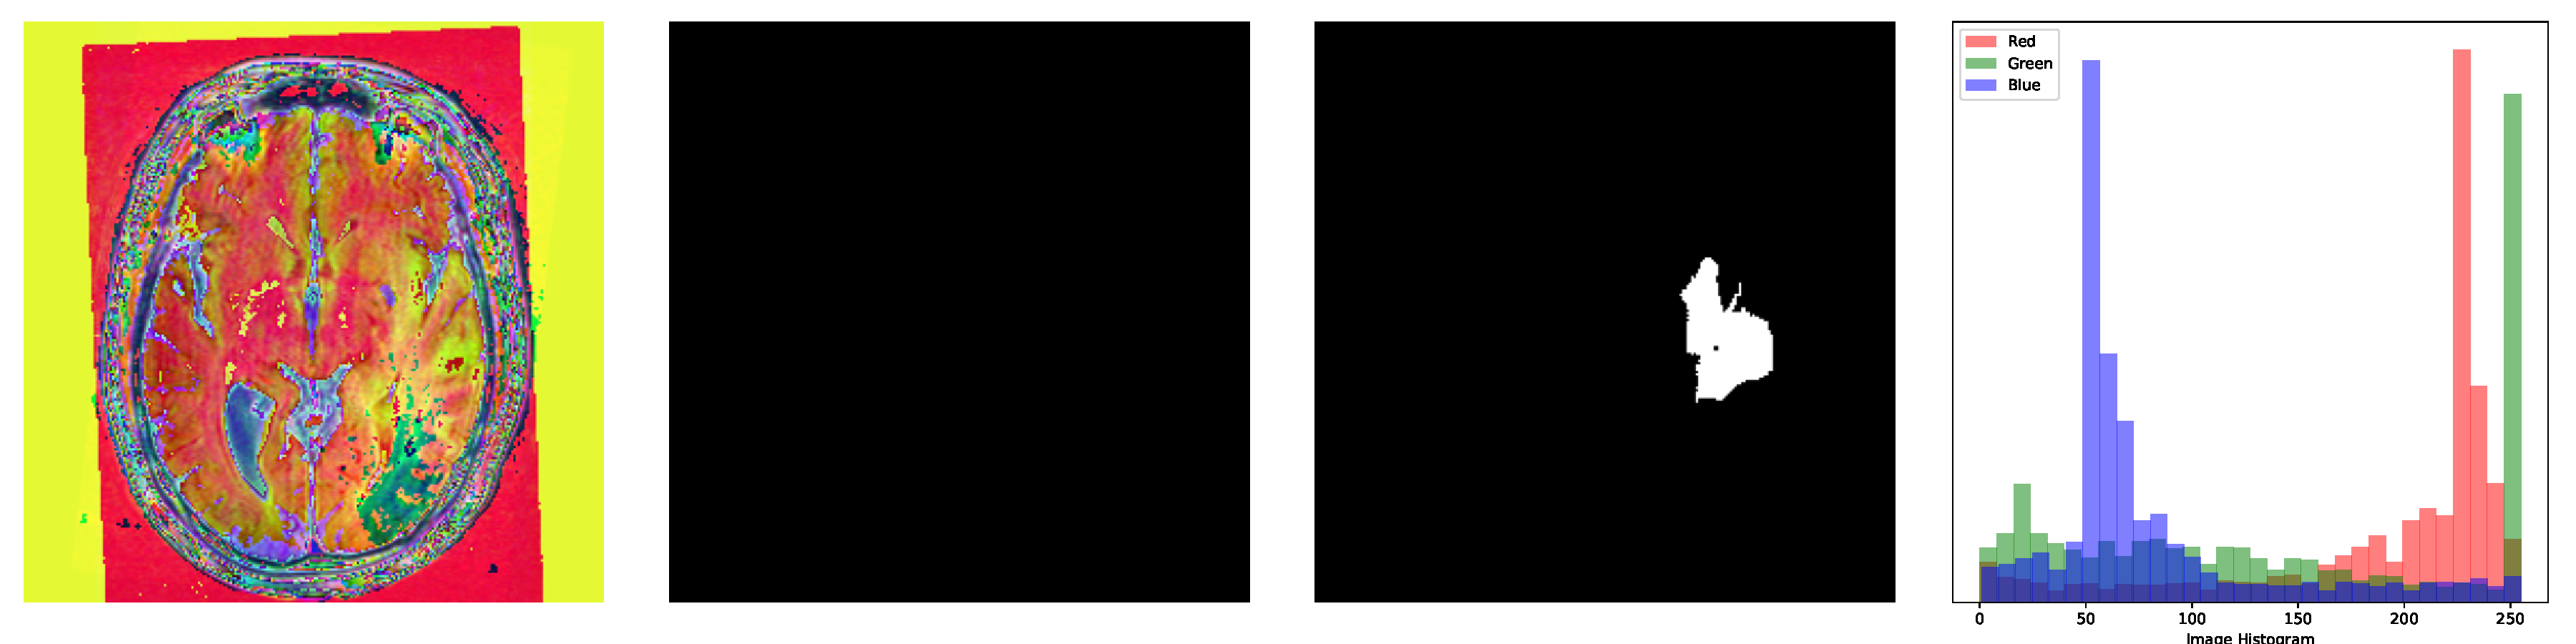
\includegraphics[width=\textwidth]{images/lab3/worst_2.pdf}
        \centering (2)
    \end{minipage}
    \begin{minipage}{0.5\textwidth}
        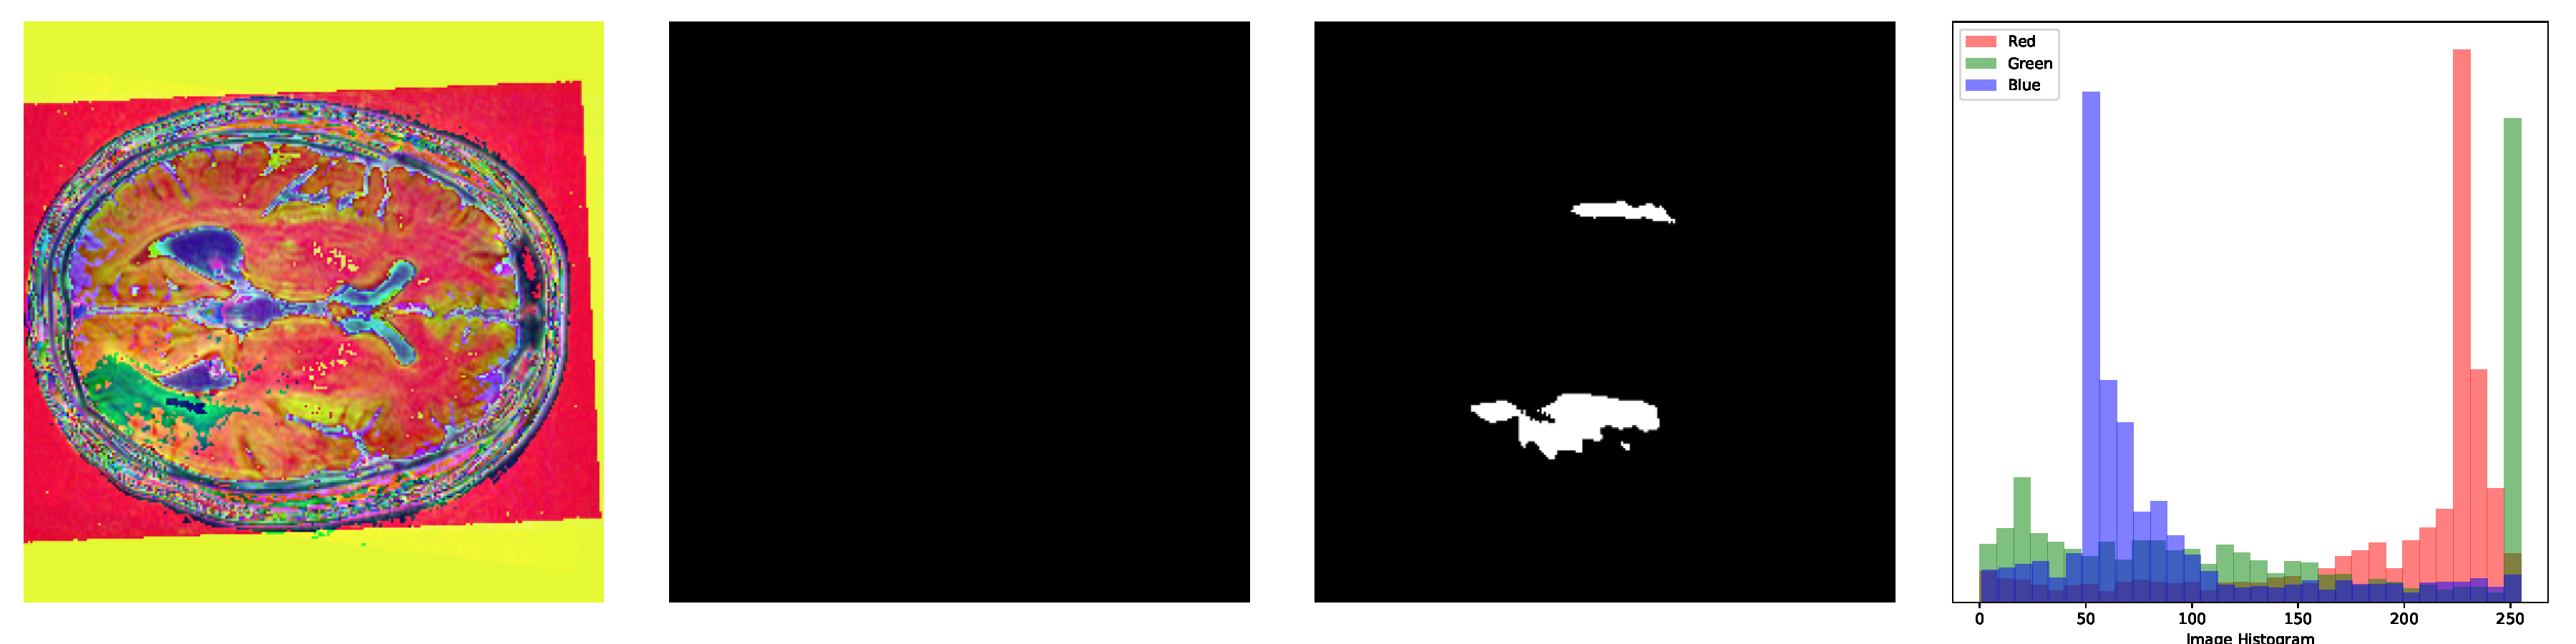
\includegraphics[width=\textwidth]{images/lab3/worst_3.pdf}
        \centering (3)
    \end{minipage}
    \begin{minipage}{0.5\textwidth}
        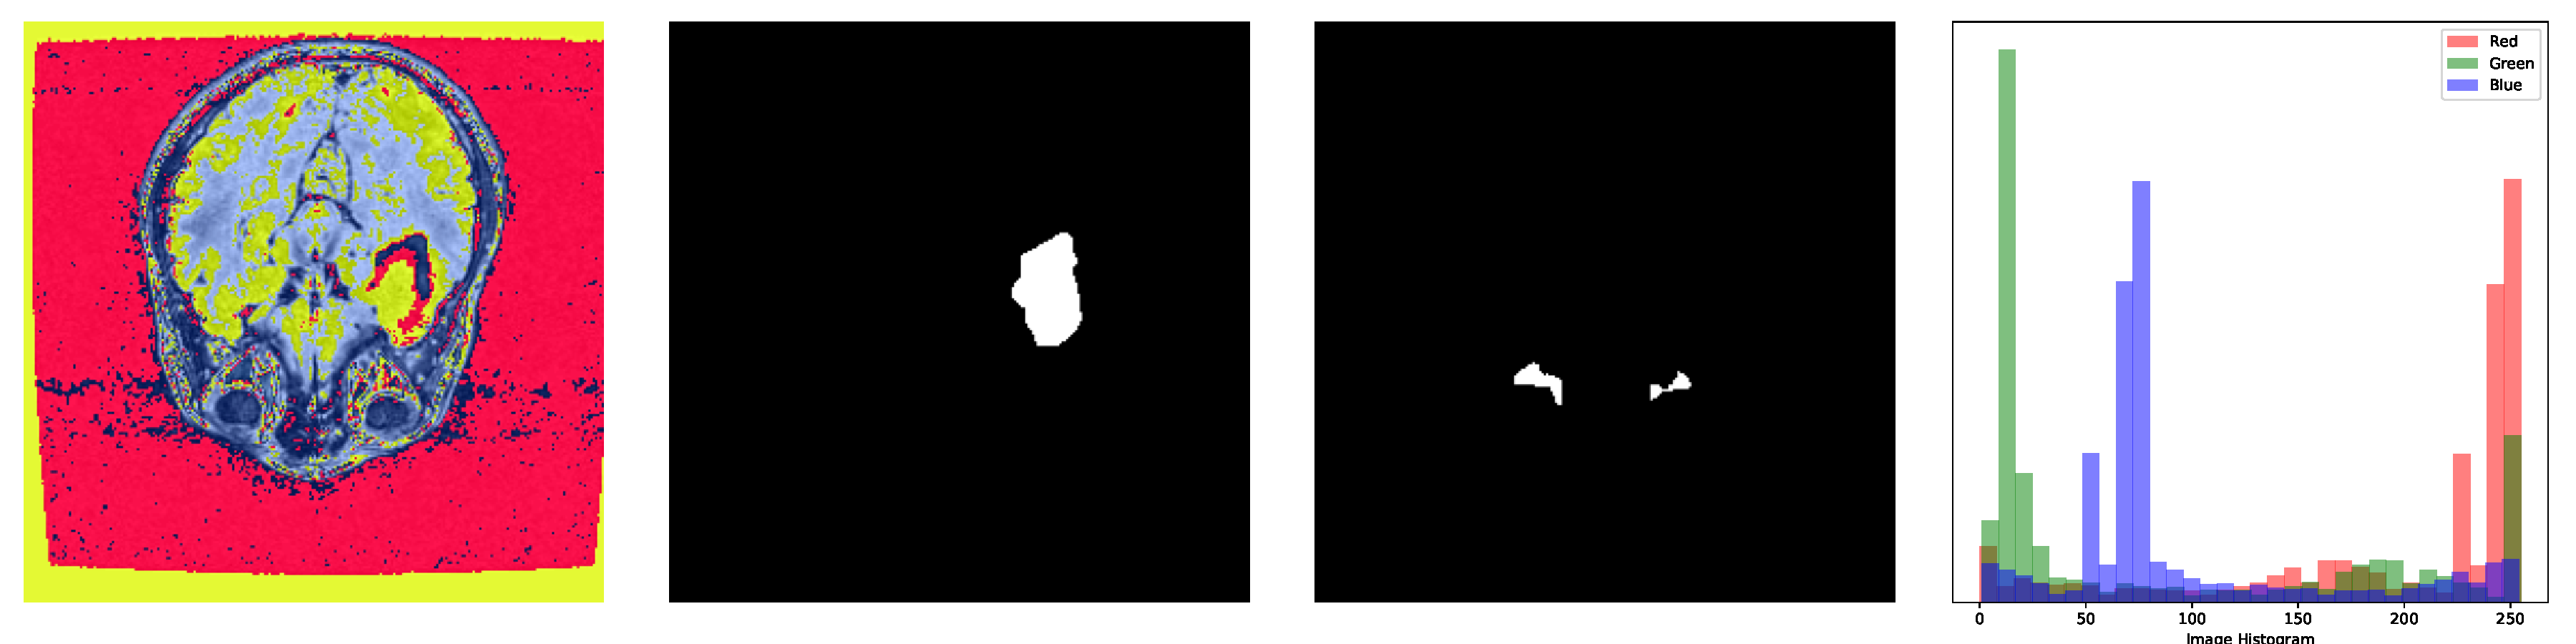
\includegraphics[width=\textwidth]{images/lab3/worst_4.pdf}
        \centering (4)
    \end{minipage}
    \begin{minipage}{0.5\textwidth}
        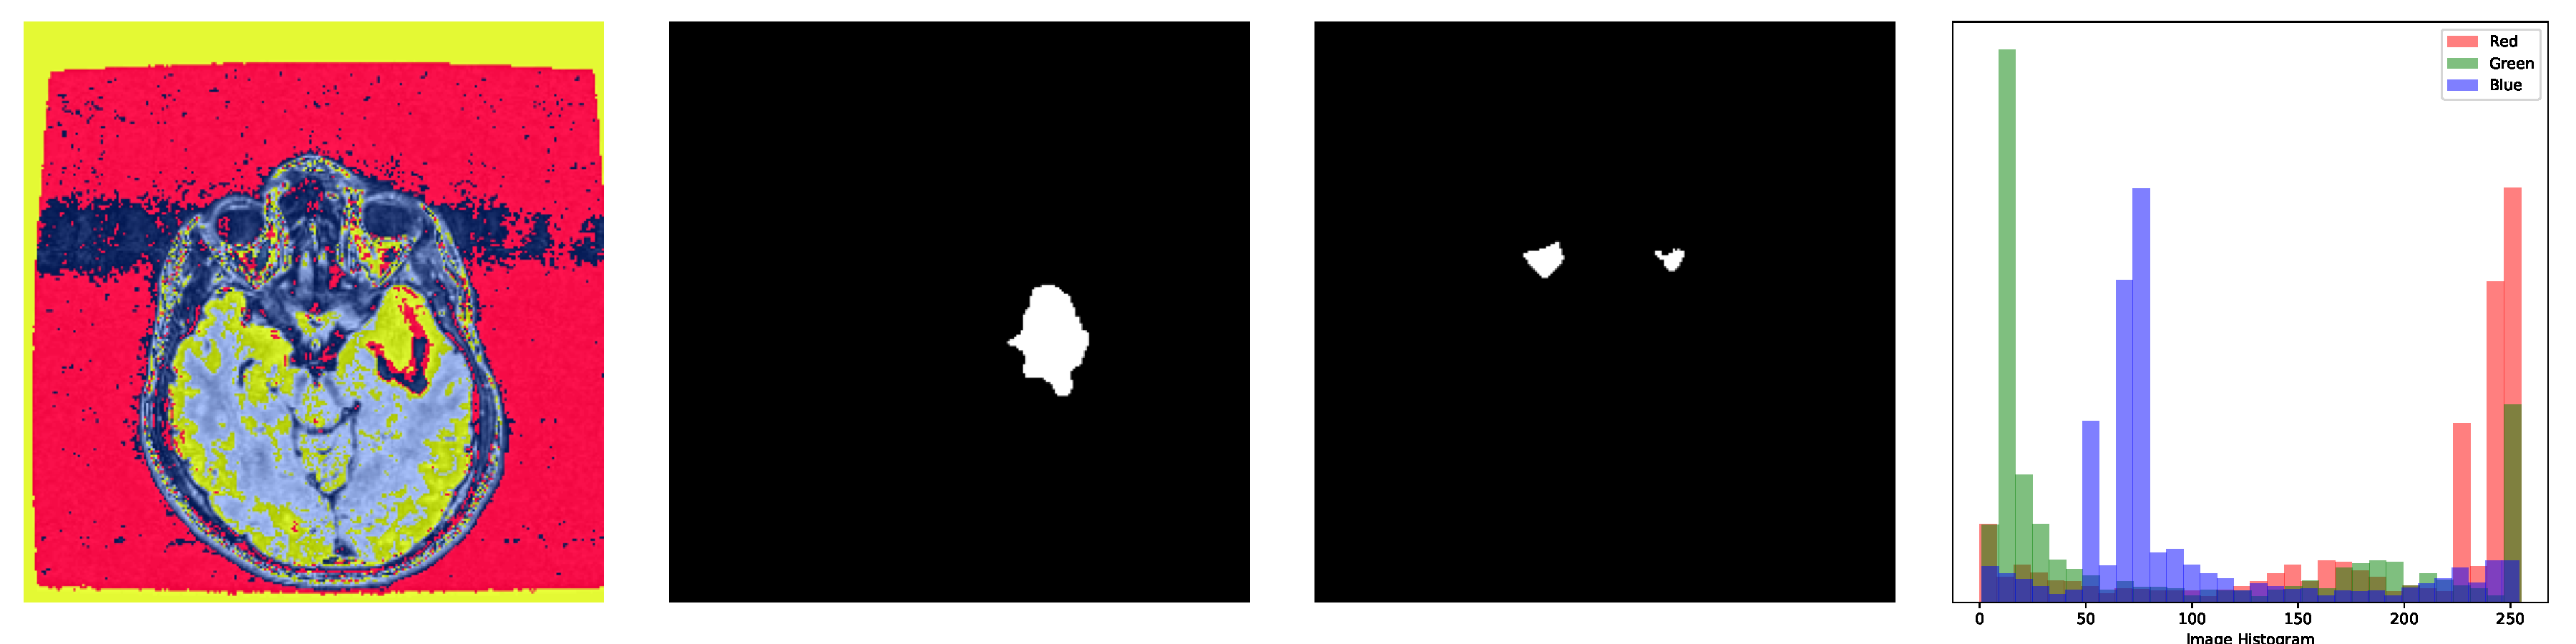
\includegraphics[width=\textwidth]{images/lab3/worst_5.pdf}
        \centering (5)
    \end{minipage}
    \caption{Worst case predictions from the U-Net model. Each subfigure shows (1)-(5): input MRI, ground truth mask, and predicted mask for the worst Dice scores. These cases highlight challenges in small object detection and boundary ambiguity.}
    \label{fig:worst_predictions}
\end{figure}




\subsection{Cross-Dataset Benchmarking}

To evaluate the generalization capability of our trained models, we performed cross-dataset evaluation on the Kvasir-SEG dataset, which contains gastrointestinal polyp segmentation images. This evaluation assesses how well models trained on brain MRI can transfer to different medical imaging domains.

\subsubsection{Kvasir-SEG Dataset Characteristics}
The Kvasir-SEG dataset contains 1,000 polyp images with corresponding segmentation masks from gastrointestinal endoscopy. Key differences from our training data include:
\begin{itemize}
    \item Different imaging modality (endoscopy vs. MRI)
    \item Color images vs. converted MRI
    \item Different anatomical structures
    \item Variable image sizes and aspect ratios
\end{itemize}



\subsubsection{Cross-Dataset Performance}
Table~\ref{tab:kvasir_results} summarizes the U-Net model's performance on the Kvasir-SEG dataset without any fine-tuning. The results show that the model failed to segment polyps in this domain, achieving a Dice score of 0.

\begin{table}[!htbp]
    \centering
    \caption{U-Net Cross-Dataset Results on Kvasir-SEG}
    \label{tab:kvasir_results}
    \begin{tabular}{lc}
        \toprule
        \textbf{Metric}  & \textbf{U-Net (No Fine-tuning)} \\
        \midrule
        Dice Coefficient & 0.000                           \\
        IoU (Jaccard)    & 0.000                           \\
        Pixel Accuracy   & 0.873                           \\
        \bottomrule
    \end{tabular}
\end{table}

Figure~\ref{fig:kvasir_predictions} illustrates representative qualitative results on the Kvasir-SEG dataset, showing that the U-Net model trained on MRI data fails to segment polyps in endoscopy images.

\begin{figure}[!htbp]
    \centering
    \begin{minipage}{0.5\textwidth}
        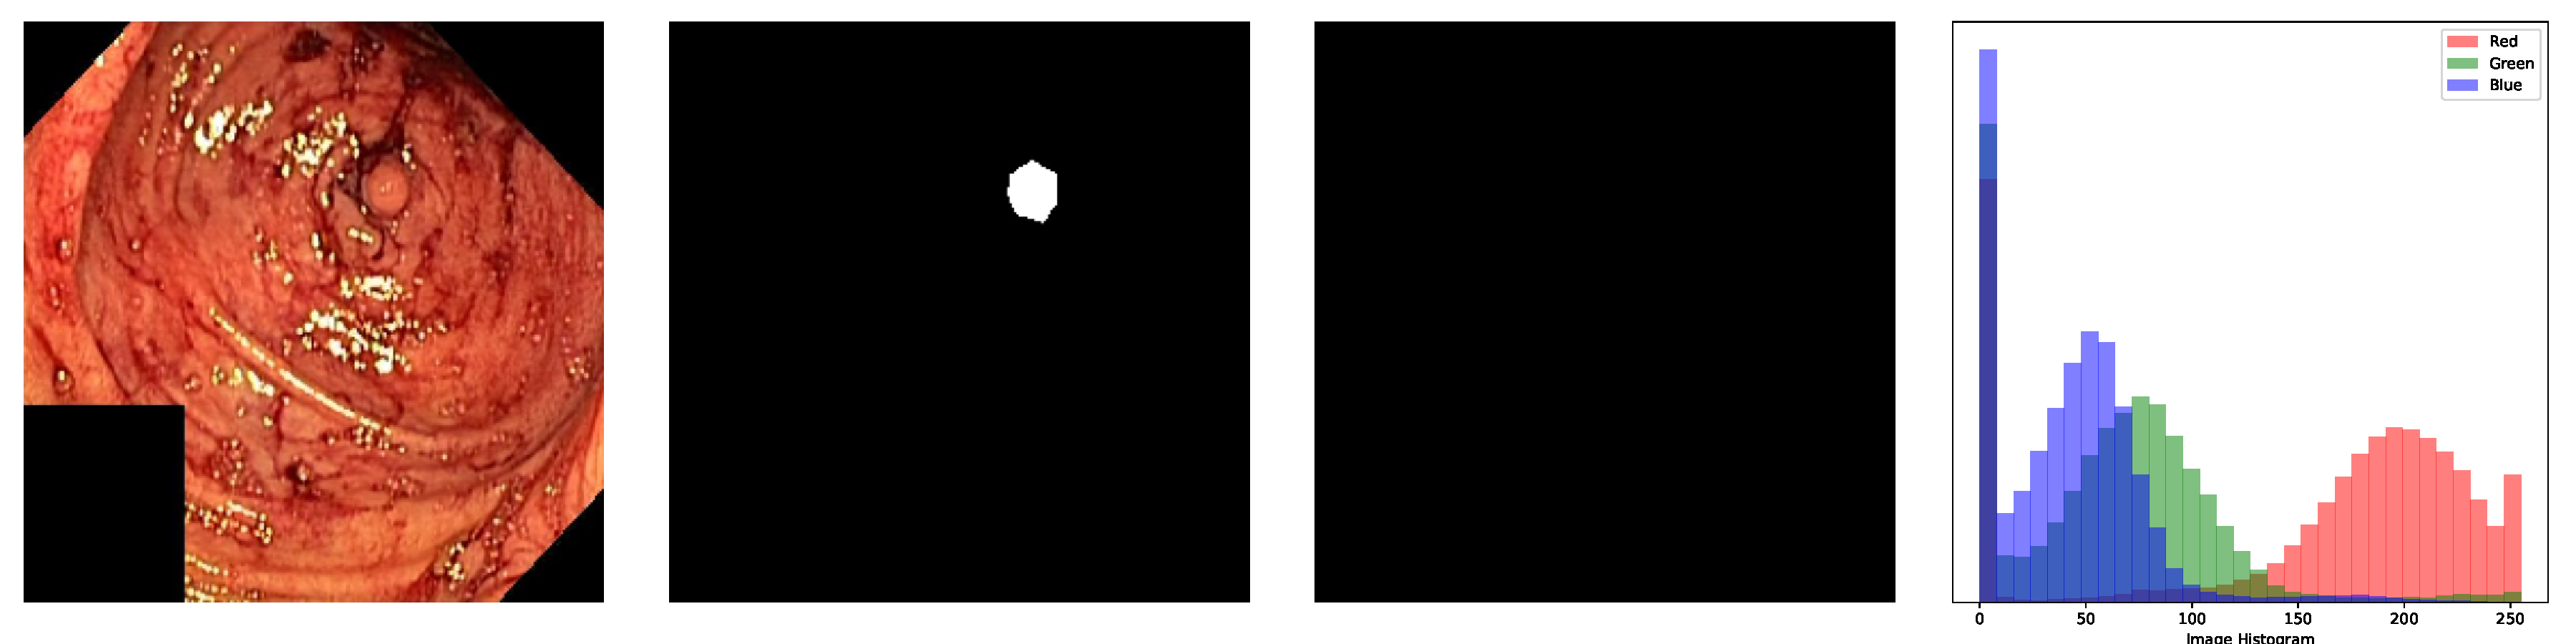
\includegraphics[width=\textwidth]{images/lab3/kvasir_1.pdf}
        \centering (1)
    \end{minipage}
    \begin{minipage}{0.5\textwidth}
        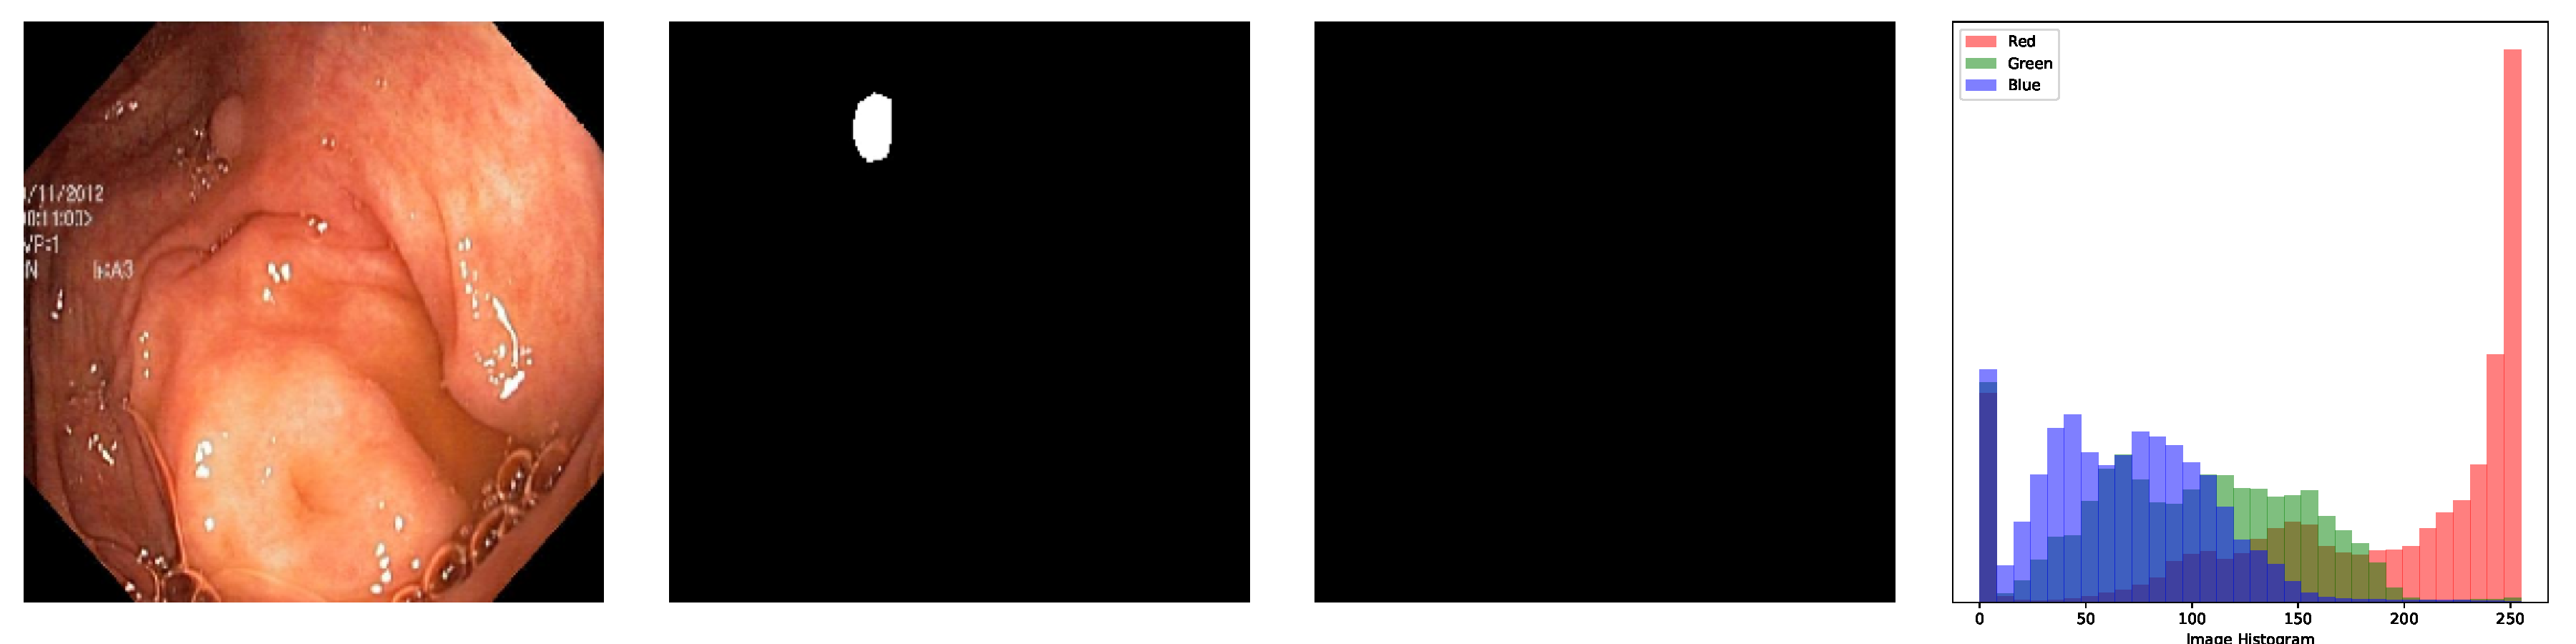
\includegraphics[width=\textwidth]{images/lab3/kvasir_2.pdf}
        \centering (2)
    \end{minipage}
    \begin{minipage}{0.5\textwidth}
        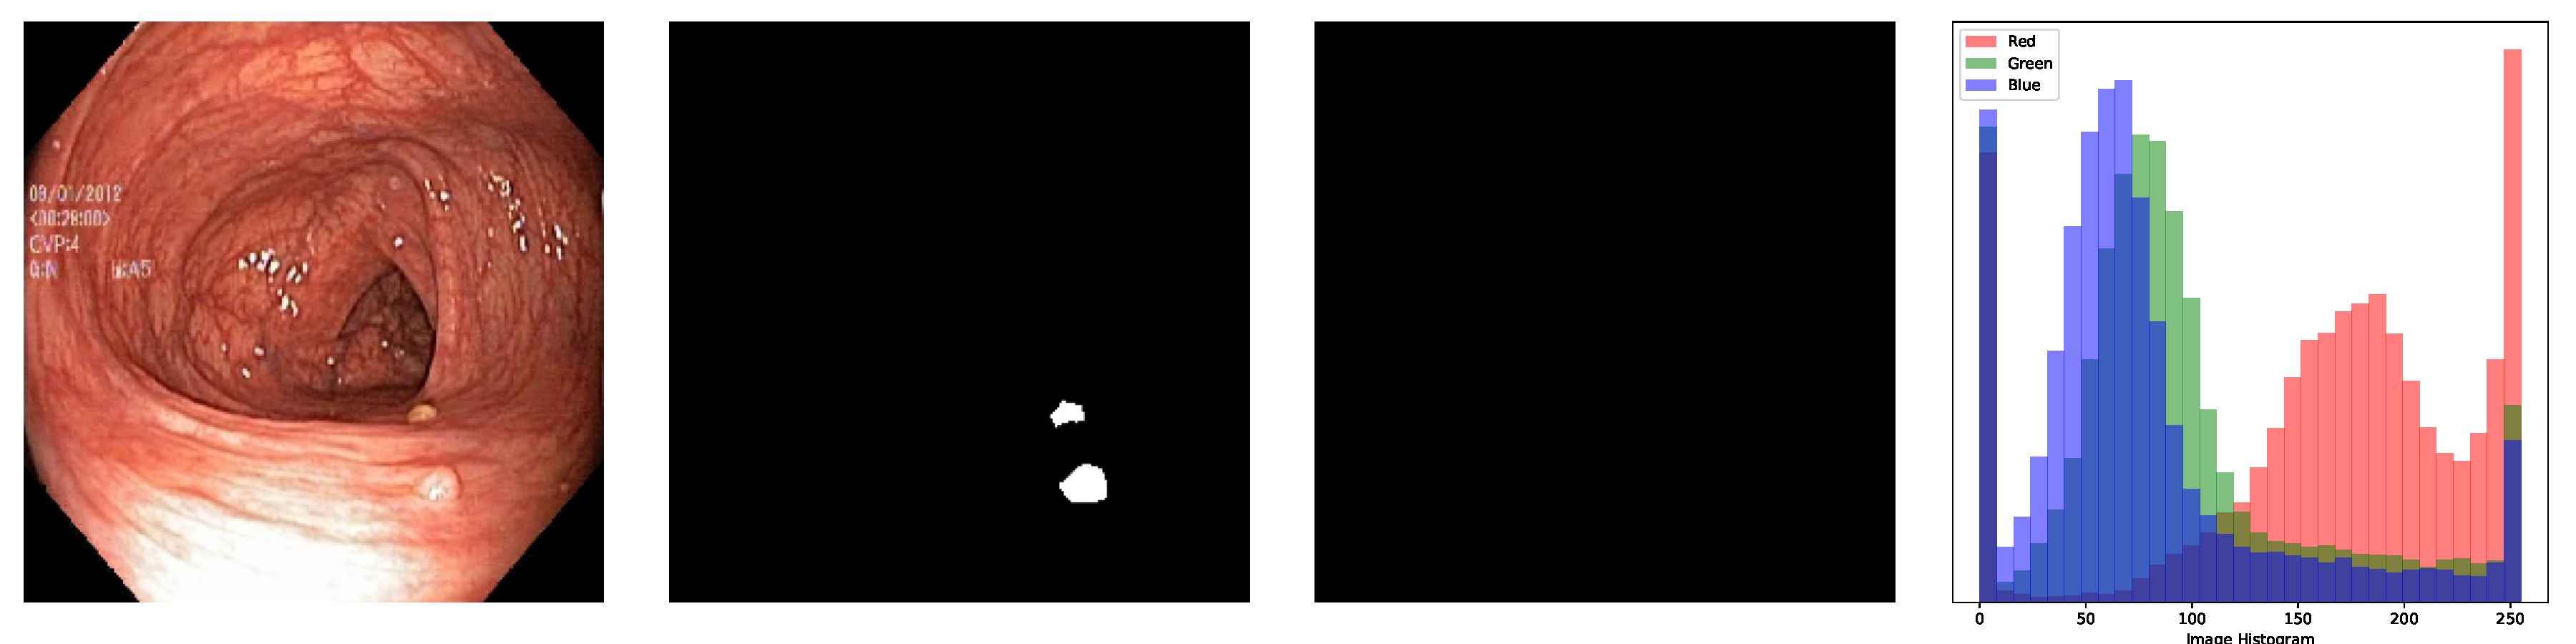
\includegraphics[width=\textwidth]{images/lab3/kvasir_3.pdf}
        \centering (3)
    \end{minipage}
    \begin{minipage}{0.5\textwidth}
        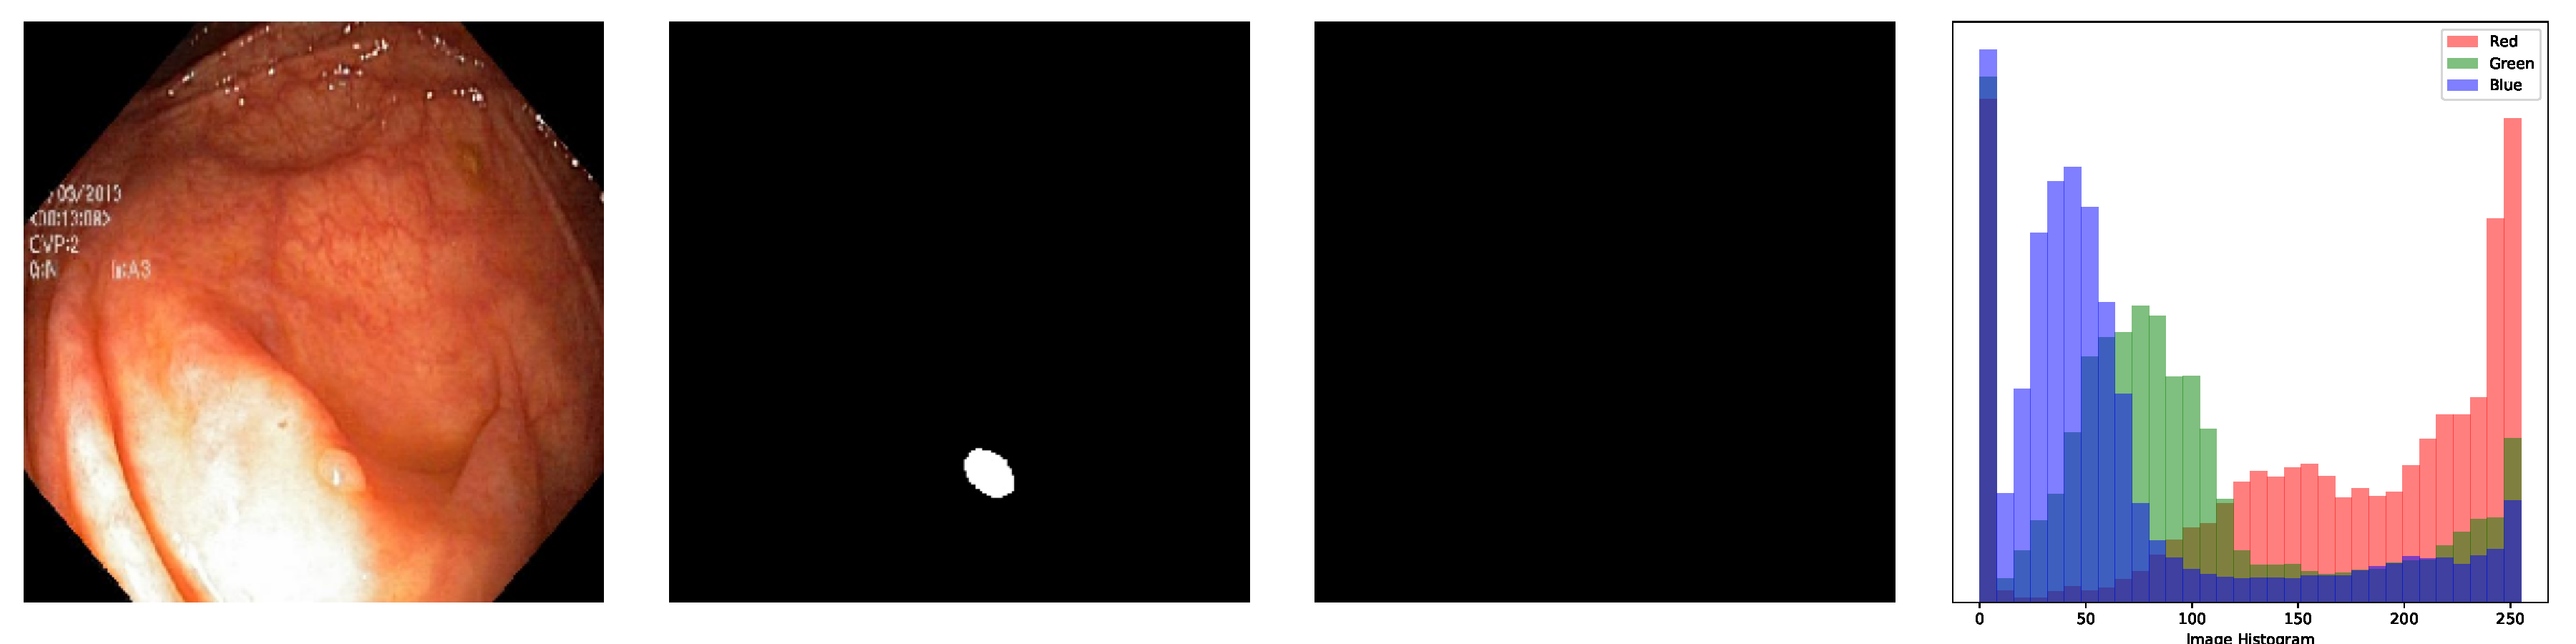
\includegraphics[width=\textwidth]{images/lab3/kvasir_4.pdf}
        \centering (4)
    \end{minipage}
    \begin{minipage}{0.5\textwidth}
        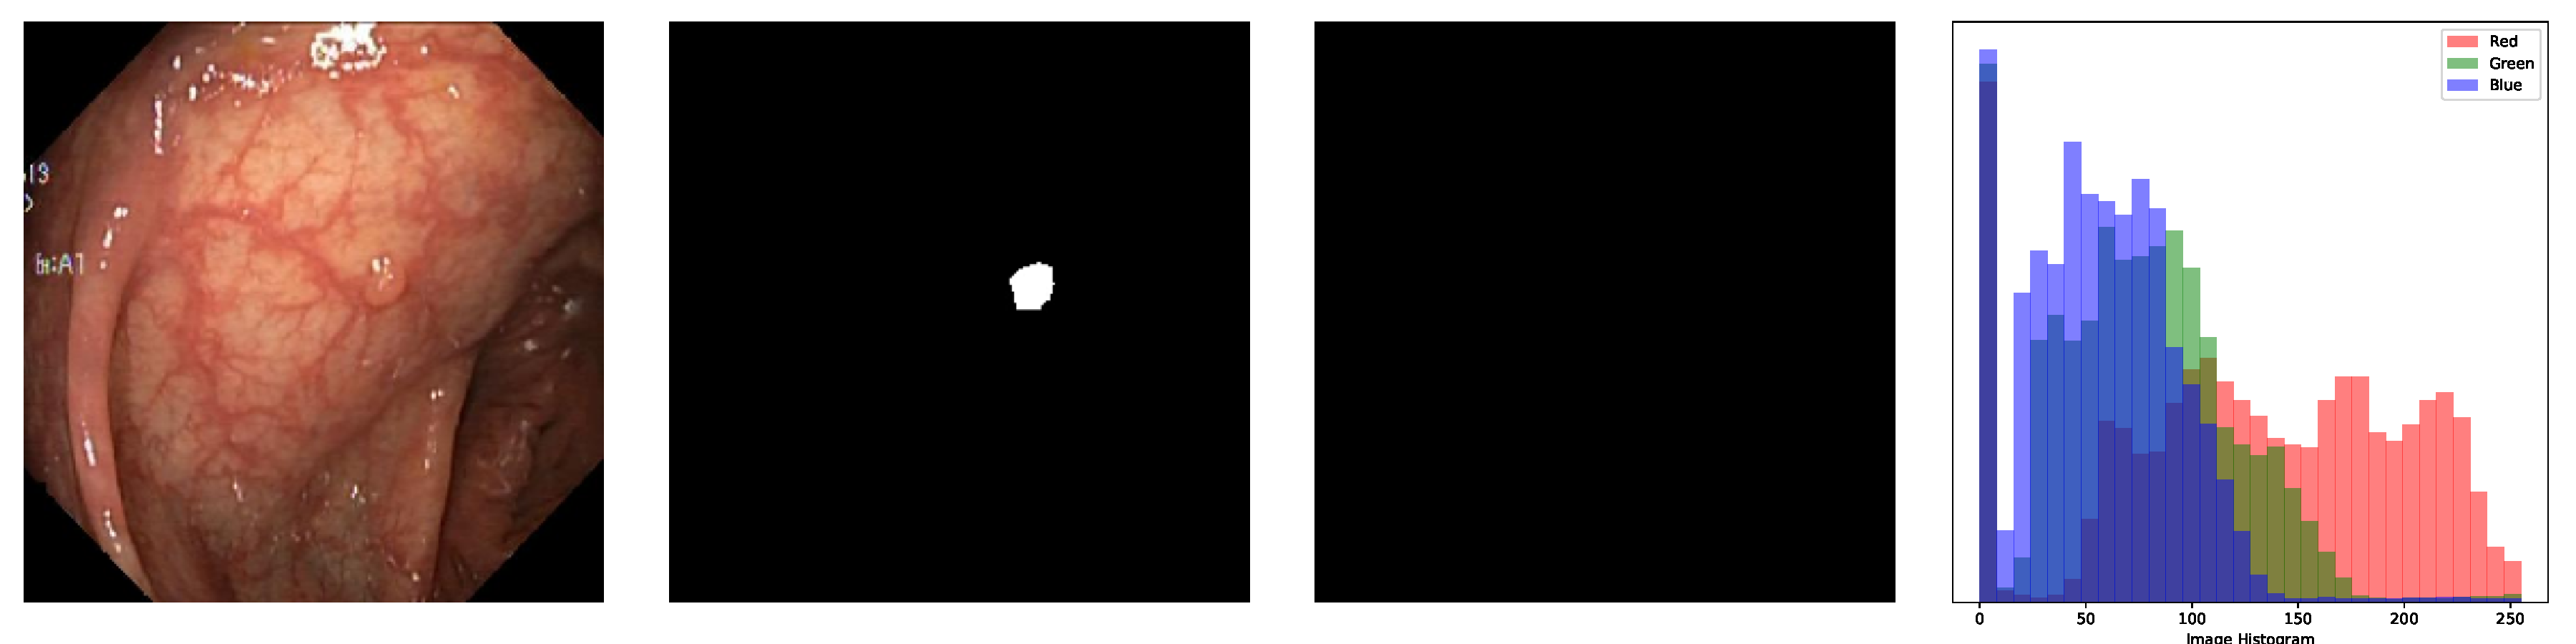
\includegraphics[width=\textwidth]{images/lab3/kvasir_5.pdf}
        \centering (5)
    \end{minipage}
    \caption{Representative Kvasir-SEG predictions from the U-Net model trained on MRI data. Each subfigure shows (1)-(5): input image, ground truth mask, and predicted mask. The model fails to segment polyps, highlighting the domain gap between MRI and endoscopy images.}
    \label{fig:kvasir_predictions}
\end{figure}


These results indicate that the U-Net model trained on MRI data does not generalize to endoscopy images without domain adaptation or fine-tuning, this might be due to the significant differences in image characteristics, small object sizes in the Kvasir-SEG dataset, and the model's reliance on features learned from brain MRI data.


\section{Conclusion}
In this study, we implemented and rigorously evaluated the U-Net architecture for brain tumor segmentation from MRI scans using the LGG dataset. Our results demonstrate that U-Net achieves high segmentation accuracy, with a Dice coefficient of 0.847 and IoU of 0.741, outperforming traditional methods and providing reliable delineation of tumor regions. The model showed robust convergence and strong performance on both quantitative and qualitative analyses, particularly excelling in cases with well-defined tumor boundaries.

However, our cross-dataset evaluation on the Kvasir-SEG dataset revealed that the model trained solely on brain MRI data does not generalize to other medical imaging modalities without further adaptation. This highlights the importance of domain-specific training and the need for transfer learning or domain adaptation techniques when applying segmentation models across different medical contexts.

Overall, our findings confirm the effectiveness of U-Net for medical image segmentation tasks, especially in scenarios with limited data and challenging class imbalance. Future work may focus on exploring advanced architectures, incorporating attention mechanisms, and leveraging multi-modal data to further enhance segmentation performance and generalizability in diverse clinical applications.

\begin{thebibliography}{20}

    \bibitem{menze2014multimodal}
    B. H. Menze et al., ``The multimodal brain tumor image segmentation benchmark (BRATS),'' \emph{IEEE Transactions on Medical Imaging}, vol. 34, no. 10, pp. 1993--2024, 2015.

    \bibitem{long2015fully}
    J. Long, E. Shelhamer, and T. Darrell, ``Fully convolutional networks for semantic segmentation,'' in \emph{Proceedings of the IEEE Conference on Computer Vision and Pattern Recognition}, 2015, pp. 3431--3440.

    \bibitem{ronneberger2015u}
    O. Ronneberger, P. Fischer, and T. Brox, ``U-net: Convolutional networks for biomedical image segmentation,'' in \emph{International Conference on Medical Image Computing and Computer-Assisted Intervention}, Springer, 2015, pp. 234--241.

    \bibitem{krizhevsky2012imagenet}
    A. Krizhevsky, I. Sutskever, and G. E. Hinton, ``Imagenet classification with deep convolutional neural networks,'' in \emph{Advances in Neural Information Processing Systems}, 2012, pp. 1097--1105.

    \bibitem{jha2020kvasir}
    D. Jha et al., ``Kvasir-SEG: A segmented polyp dataset,'' in \emph{International Conference on Multimedia Modeling}, Springer, 2020, pp. 451--462.

\end{thebibliography}

\end{document}
\bibitem{jha2020kvasir}
D. Jha et al., ``Kvasir-SEG: A segmented polyp dataset,'' in \emph{International Conference on Multimedia Modeling}, Springer, 2020, pp. 451--462.

\end{thebibliography}

\end{document}
